% TRUTH VERSION: elite_status-v01.tex
% FILE ROLE: AUTHORITATIVE SOURCE
% DOCUMENT: Economics Journal Draft


\documentclass[12pt,letterpaper]{article}
\usepackage[utf8]{inputenc}
\usepackage{amsmath,amssymb,amsthm}
\usepackage{graphicx}
\usepackage{natbib}
\usepackage{booktabs}
\usepackage{setspace}
\usepackage{geometry}
\usepackage[colorlinks=true,citecolor=blue,linkcolor=blue]{hyperref}
\geometry{margin=1.1in}

\newtheorem{theorem}{Theorem}
\newtheorem{proposition}{Proposition}
\newtheorem{lemma}{Lemma}
\newtheorem{corollary}{Corollary}
\newtheorem{assumption}{Assumption}
\newtheorem{remark}{Remark}
\theoremstyle{definition}
\newtheorem{definition}{Definition}

\newcommand{\Lists}{\Lambda}
\newcommand{\R}{\mathbb{R}}

\title{The Market for Elite Status\thanks{Working draft --- not for circulation.
The algebraic derivations and numerical examples in the appendices are verified in companion code (\texttt{analysis/} in the project repository); qualitative claims are proven in the text, with example-specific verifications labeled as such.}}
\author{Jo\~{a}o Ricardo Faria\\ Florida Atlantic University
  \and Michael D. Ryall\\ Florida Atlantic University}
\date{\today}

\begin{document}

\maketitle

\begin{abstract}
\noindent Prosperity, on an influential recent account, breeds elite overproduction: the class of leaders and managers expands, its institutions absorb growing resources, and the surplus returned to society shrinks --- a diagnosis that now animates hostility toward elites and elite institutions across the political spectrum.
The private-sector rejoinder is that free markets provide the check: managers selected for pedigree rather than productivity will run inefficient firms, and competition will squeeze them out.
We price elite status itself --- admission to an elite school, then command of an elite firm --- in a competitive general-equilibrium economy, and show that the rejoinder fails in an exact way.
Competition does eliminate any institution dominated in the complete product it sells, status included: a rival supplying equivalent standing at lower resource cost would displace the elite system in every equilibrium.
But a rival that is merely more productive need not displace anything, because it does not sell what elite participants are buying.
The drain is therefore real --- when the elite complex returns less output per unit of resources, aggregate output falls as the taste for status spreads --- yet it is no wealth pump: elite managers earn visible salary premia but accept lower payoffs net of elite education, and this status discount finances the entire system at market prices.
Every such equilibrium is Pareto optimal, so there is nothing for markets or policy to correct --- unless status is valued for its scarcity, in which case entry dilutes incumbents, over-entry results, and a corrective membership tax can raise welfare and output together, as it does in our example.
Dynamically, richer societies support larger elites --- elite overproduction as a luxury --- and our example economy converges, knowingly, to permanently lower wealth than its status-free counterfactual.
\medskip
\noindent\textbf{Keywords:} elite status; clubs; general equilibrium; positional externalities; credentialism; elite overproduction.\\
\textbf{JEL codes:} D51, D62, D71, I24, J31, Z13.
\end{abstract}

\onehalfspacing

\section{Introduction}\label{sec:intro}

In \emph{End Times}, the historian Peter Turchin argues that societies at a certain stage of development begin to overproduce elites: the class of leaders and managers expands beyond the positions available to it, turns away from its shepherding role, and constructs ``wealth pumps'' that enrich elites at the expense of everyone else \citep{turchin2023endtimes}.
Whatever one makes of the historiography, the sentiment has constituencies: significant political movements across the globe now organize around hostility toward elites and the institutions that produce them.

For the private sector, at least, there is a natural rejoinder: free markets provide the check.
Managers selected for pedigree rather than productivity will run inefficient firms; an institution that consumes more resources than it returns should be undercut by rivals; over time, competition squeezes the incompetent and the self-serving out.
The rejoinder has a problem, and it is not theoretical.
Elite schools and the firms their graduates run have not been competed away; they have persisted, and expanded, through decades of intense competition in product, labor, and education markets.

Part of the reason lies in what these institutions actually sell.
Elite institutions absorb ever more resources per graduate, and how much of what they sell is skill remains contested: for the average admitted student, attending a more selective college adds little to earnings once student quality is held fixed \citep[with the notable exceptions of disadvantaged students, and with returns tracking college resources]{dalekrueger2002}; the causal payoff of elite programs accrues disproportionately to the already advantaged --- in Chile, entirely to men from elite private high schools \citep{zimmerman2019elite}; admission to Ivy-Plus colleges operates through gateways to prestigious firms and graduate schools \citep{chettydemingfriedman2026}; and among interwar Harvard students the labor-market premium to joining the right social clubs exceeded, descriptively, the premium to academic performance \citep{michelmanpricezimmerman2022}.
The firms that recruit preferentially from these institutions screen on pedigree and polish as much as on tested ability \citep{rivera2015pedigree}.

This paper shows that markets do work here --- but the check they run is not the one the rejoinder imagines, and material efficiency is not what it delivers.
The displacement argument orders institutions by their material output; the market trades complete products, and the product of an elite institution includes a membership.
We model elite status as what it observably is: a membership, first in a school and subsequently in the class of people who run certain firms, that is bought and sold at market prices.
The natural home for such a model is the general equilibrium theory of clubs developed by \citet{ellickson1999clubs,ellickson2001clubs,ellickson2006organization}, in which group memberships are priced alongside ordinary commodities and agents care about the characteristics of their fellow members.
Within that framework we obtain four results.

First, and organizing the rest, a displacement theorem draws the boundary the familiar argument leaves implicit (Theorem~\ref{thm:displacement}).
Competition does eliminate dominated institutions, in the following exact sense: a group type with a feasible \emph{membership-equivalent} replacement --- one whose seats carry the same qualifications and the same utility for their holders --- at lower resource cost cannot be active in any equilibrium.
What competition does not act on is material dominance alone: an institution can lose every material comparison and survive in the strong core, because the comparison omits the membership its members are paying for.
The boundary is visible inside the model itself.
The serious school undercuts the elite school's cost and supplies the same amenity, and fails to displace it for exactly one reason: its degree does not confer the elite qualification.
The elite premium prices the qualification, not the classroom.

Second, equilibrium compensation reproduces the gross configuration compensation data show and pairs it with a net prediction those data do not yet test.
Elite managers earn a gross wage premium over their competently trained peers, pinned by their firms' revenue; net of education costs, however, they accept a strictly lower payoff --- the status discount that finances the system (Corollary~\ref{cor:wages}).
The premium decomposes exactly (gross premium equals excess tuition minus the status discount), so the status-financed component of elite pay is tuition reimbursement rather than productivity, and the decomposition yields the model's sharpest prediction: changes in elite tuition have zero incidence on elite salaries, being absorbed by the status discount.
The waste is thus financed by identified parties at market prices; no friction, information asymmetry, or market power is involved.
The incidence is the reverse of a wealth pump: the elite do not extract the system's cost from the rest of society; they pay it.
The same accounting yields a sharp possibility theorem: even \emph{strictly less productive} elite firms survive whenever the status discount exceeds the workers' compensating differential plus the resources burned (Proposition~\ref{prop:coexist}) --- though in that polar case the gross premium necessarily reverses, so the empirically relevant configuration is the one in which elite firms are more productive per firm and their managers visibly better paid.

Third, as the taste for status spreads through the population, aggregate output falls monotonically (Proposition~\ref{prop:decline}).
What matters is not productivity per firm but output \emph{per unit of resources consumed}: in our central configuration elite firms produce strictly more output than competent ones, look superior in any firm-level comparison, pay their managers more --- and still drag aggregate output down, because the elite school system burns resources that firm accounts never show.

Fourth, every such equilibrium lies in the core of the economy and is Pareto optimal (Theorem~\ref{thm:nocorrection}).
No coalition of agents, deploying the economy's group types in any configuration, can achieve a Pareto improvement.
The market has nothing to correct: falling aggregate output is the equilibrium price of status consumption.
The popular syllogism ``markets work, therefore materially wasteful institutions cannot survive competition'' commits a non sequitur, and Theorem~\ref{thm:displacement} locates it precisely: the syllogism is valid for complete products and invalid for their material projections.

The efficiency of the baseline is not a celebration; it is a diagnosis.
Within the environments we model, it locates where a genuine market failure must live: not in the waste, which is priced, but in the \emph{relativity} of status.
Section~\ref{sec:positional} makes status positional (valuable because others lack it) so that each entrant into the elite dilutes the status of every incumbent.
This economy-wide externality lies outside the assumptions of the clubs welfare theorems: membership prices internalize composition effects \emph{within} a group, but eliteness is a characteristic of a class that spans all elite groups.
The positional equilibrium exists, is unique, and self-limits (dilution shrinks the elite), but it is no longer Pareto optimal and no longer in the core (Propositions~\ref{prop:positional} and~\ref{prop:inefficiency}): there is over-entry into elite institutions (Proposition~\ref{prop:tax}), and a corrective membership tax can raise welfare and output together, as it does in our example.
The contrast between Theorem~\ref{thm:nocorrection} and Proposition~\ref{prop:inefficiency} is the paper's answer to when elite waste is and is not a policy problem: absolute status is efficient consumption; positional status is a rat race.

Section~\ref{sec:dynamics} sets the economy in motion.
Each generation inherits the resources its parents saved, plays the club economy within its lifetime, and bequeaths; the static model is the period economy and its comparative statics become the transition map.
A single condition (the one already governing the static output decline) delivers two further results.
Status is a luxury in equilibrium: because the elite sector's waste is a fixed resource cost while wages scale with wealth, richer economies support larger elites (Proposition~\ref{prop:luxury}).
This is elite overproduction, delivered by prices rather than by capture.
And the elite sector drags on accumulation: rising wealth expands the status spending that absorbs it, and the steady state settles permanently below the status-free counterfactual (Proposition~\ref{prop:drag}, under single-crossing provisos our example satisfies) --- with no collapse, because falling wealth prices the elite out of existence before it can extinguish the economy.
The path involves no error and no myopia: it is common knowledge, and no atomistic parent could or would deviate.
Nor does the conclusion rest on parents who fail to look ahead: within a degree-one preference class, any common savings motive, forward-looking or not, changes how much a generation saves but never how the market for status operates at a given wealth (Proposition~\ref{prop:invariance}).
Rational societies really do let it happen.

Three features distinguish the exercise from prior work, which Section~\ref{sec:lit} reviews in detail.
Status here is \emph{produced and sold} by institutions with real resource costs and competitively priced as a club membership, rather than attached to occupations, allocated by norms, sold by a monopolist, or traded as an abstract good in fixed supply.
The persistence result is at the level of the \emph{firm}, with the financing of elite inefficiency traced to identified parties at market prices.
And the welfare analysis is disciplined by the framework's own theorems, so that both boundaries the paper draws --- between what competition eliminates and what it sustains, and between efficient status consumption and a genuine rat race --- are theorems, not stances.

The paper proceeds as follows.
Section~\ref{sec:lit} positions the contribution.
Section~\ref{sec:framework} presents the general framework and Section~\ref{sec:model} our economy.
Section~\ref{sec:equilibrium} characterizes equilibrium, the compensation decomposition, the no-market-correction theorem, and the displacement boundary, illustrated numerically in Section~\ref{sec:example}.
Section~\ref{sec:positional} develops the positional extension and Section~\ref{sec:dynamics} the overlapping-generations dynamics.
Section~\ref{sec:empirics} collects the model's empirical content, Section~\ref{sec:discussion} discusses interpretation and extensions, and Section~\ref{sec:conclusion} concludes.
All derivations are gathered in the appendices and are verified symbolically in the paper's companion code.

\section{Related Literature}\label{sec:lit}

\textbf{Markets for status.}
The idea that status itself can be traded has an established lineage.
\citet{beckermurphywerning2005} price status as a divisible good in fixed supply traded in a hedonic market alongside consumption; their central objects are the induced income distribution and the complementarity between status and consumption.
We differ in making the supply side explicit: status here is membership in clubs (schools and the firms their graduates run) produced by institutions with real resource costs and priced by the membership prices of \citet{ellickson1999clubs}, with a full production economy attached, so that the resource cost of status and its incidence across workers, managers, and schools are equilibrium objects rather than primitives.
\citet{colemailathpostlewaite1992} generate status-driven distortions from self-enforcing matching norms, in which rank governs access to nonmarket goods; our status is marketed rather than normed, which yields prices, entry margins, and comparative statics that norms models do not deliver, at the cost of taking the taste for membership as a primitive.
A third tradition studies a single designer selling status: contest categories in \citet{moldovanuselashi2007}, exclusive groups with peer effects in \citet{board2009group}, pure signals of type in \citet{rayo2013signal}, and the fashion cycles of \citet{pesendorfer1995fashion}, in which an intrinsically useless good profitably sorts its buyers.
Here, by contrast, the supply of status is competitive (any potential group type is priced) and embedded in general equilibrium, which is what allows welfare statements about the whole economy rather than about a designer's profit.
Conspicuous-consumption signaling \citep{bagwellbernheim1996veblen} shares our subject but not our mechanism: our economy has no hidden types, so the persistence of elite waste cannot be attributed to information.

\textbf{Status and allocation.}
\citet{fershtmanmurphyweiss1996} show occupational status concerns distort the allocation of talent in growth.
Our persistence result is at the level of the \emph{firm}: identifiable, resource-inefficient organizations survive (even output-inferior ones can) because their control rights are bundled with status consumption.
The rat-race tradition (\citealt{akerlof1976caste}; \citealt{hopkinskornienko2004}; \citealt{frank1985demand}; \citealt{hirsch1976social}) delivers genuine inefficiency from relative comparison; in our baseline there is no externality and hence no rat race --- that distinction is the point of Theorem~\ref{thm:nocorrection}, and Section~\ref{sec:positional} shows exactly what must be added to overturn it, using the widespread-externalities equilibrium concept of \citet{noguchizame2006externalities}.
\citet{kimtertiltyum2024} provide a recent quantitative treatment of education-status externalities; we provide the institutional theory.

\textbf{Education and elite institutions.}
In \citet{spence1973signaling} education is privately valuable because it is informative about hidden types.
Our elite school conveys no information (there are no hidden types anywhere in the model) and its product is the membership itself; the mechanism would survive full information, which cleanly separates it from signaling.
This places us closest to the reputation-and-selection view of schooling of \citet{macleodurquiola2019}, in which schools are valued for whom they admit rather than what they teach, and to the empirical literature finding that elite institutions' value operates through access and affiliation rather than measured skill production: selectivity premia near zero for the average admitted student \citep{dalekrueger2002}, elite-program returns concentrated on the already advantaged \citep{zimmerman2019elite}, social-club premia exceeding academic premia \citep{michelmanpricezimmerman2022}, admission effects operating through gateways to prestigious firms \citep{chettydemingfriedman2026}, and hiring at elite professional-service firms screening on pedigree \citep{rivera2015pedigree}.
We treat the zero-teaching elite school as a polar case; \citet{arteaga2018} shows curricular content matters even at a top university, and nothing in our results requires the polar case (Remark~\ref{rem:polar}).

\textbf{The clubs framework.}
Our machinery descends from \citet{buchanan1965clubs} through the competitive general-equilibrium formulation of \citet{ellickson1999clubs,ellickson2001clubs,ellickson2006organization}; \citet{scotchmer2002clubs} surveys the field, \citet{coleprescott1997valuation} provides the lottery formulation, and \citet{allouchwooders2008} relax the bounds on club sizes.
Applied uses of this machinery are rare: the main exceptions are \citet{caucutt2001peer,caucutt2002vouchers}, who compute club equilibria of school economies with peer effects, and the firms-as-clubs analyses of \citet{prescotttownsend2006firms} and \citet{zame2007incentives}, the latter establishing that with strategic play inside firms, equilibria may be Pareto ranked.
To our knowledge the present paper is the first to use the framework to price status and the first to embed a widespread externality in it; we are also not aware of prior work studying transition dynamics whose period-by-period allocations are club equilibria, though computed club economies of schooling \citep{caucutt2001peer,caucutt2002vouchers} come closest.

\textbf{Dynamics.}
The rent-seeking-and-decline tradition (\citealt{murphyshleifervishny1991}; \citealt{baumol1990entrepreneurship}; \citealt{acemoglu1995reward}) diverts talent to unproductive activity through distorted rewards; our drag operates instead through competitively priced status consumption, and its strength is disciplined by the same condition that governs the static equilibrium.
Where \citet{hasslermora2000} and \citet{colemailathpostlewaite1992} sustain aristocratic regimes through information or norms, our elite is sustained by prices --- and where the leisure-loving aristocracies of \citet{doepkezilibotti2008} are competed away at industrialization, ours survive precisely because their inefficiency is financed by willing status buyers rather than borne by the firms' bottom line.
The memberships tradition in inequality dynamics (\citealt{durlauf1996persistent}; \citealt{galorzeira1993}) generates traps from productive group memberships and credit constraints; our membership is a pure positional good, and our poverty dynamics run top-down (wealth creates the elite that erodes wealth) rather than bottom-up.
Finally, the pattern our dynamics formalize, prosperity breeding an expanding elite that strains the society supporting it, is the ``elite overproduction'' of \citet{turchin2023endtimes}.
That literature is historical and demographic; to our knowledge, no formal treatment with optimizing agents and market-clearing prices exists, and Propositions~\ref{prop:luxury} and~\ref{prop:drag} may be read as one.

\section{The Framework}\label{sec:framework}

We adopt the general equilibrium model of groups of \citet{ellickson2006organization}, which extends \citet{ellickson1999clubs} to allow groups to produce outputs and memberships to carry acquired characteristics.
This section states the primitives, explains what each is intended to represent, and records the two theorems we use; the reader is referred to the source for proofs and for the framework's full generality.

\paragraph{Notational conventions.}
Throughout the paper, lowercase Latin and Greek letters denote parameters, functions, and elements of sets; capital Latin and Greek letters denote sets; and calligraphic letters denote collections of sets (the only instance below is a $\sigma$-algebra).
Blackboard letters denote the standard number systems: $\R$ is the real line, $\R^N$ its $N$-fold Cartesian product, $\R_+$ the nonnegative reals, and $\mathbb{Z}_+=\{0,1,2,\dots\}$ the nonnegative integers.
Two standard exceptions are retained: distribution functions are written with the conventional capital $F$, and a bar over a lowercase letter ($\bar{w}$, $\bar{y}$) denotes an economy-wide aggregate of the corresponding individual quantity.
Every symbol is defined where it first appears.
Two workhorse letters serve double duty across distant contexts where no ambiguity can arise: $s$ is an organizational characteristic in the group-type notation and the taste-scale parameter of the numerical examples, and $t$ is the membership tax of Section~\ref{sec:positional} and the time index of Section~\ref{sec:dynamics}.
Bars also mark two bounds ($\bar\ell$, $\bar\eta$) alongside the aggregates; the count $N$, utilitarian welfare $W$, the appendix aggregator $A$ and its common factor $Q$, and the rebate level $T$ are capitals by long convention; the letter $m$ names both generic memberships (always paired with a group type or subscripted) and the elite mass of Section~\ref{sec:positional}; and $b$ is the warm-glow bequest of Section~\ref{sec:dynamics} and, in the magnitude exercise of Section~\ref{sec:empirics}, the burn share.

\subsection{Commodities, groups, and memberships}

There are $N\geq 1$ perfectly divisible, publicly traded private goods; a bundle of them is a vector in $\R^N$.
Alongside these ordinary commodities, the framework's distinctive objects are \emph{groups}: collections of individuals associated for some purpose --- in our application, schools and firms.

Two exogenous finite sets describe the raw material from which groups are built.
$\Omega$ is the set of \emph{membership characteristics}, with typical element $\omega$.
A membership characteristic is any attribute of a person that matters to the group she joins or to the activity conducted there: a role (student, laborer), a qualification (holding a particular degree), or a position (manager).
Characteristics are observable and contractible, and (importantly for what follows) they can be \emph{acquired}: attending a school confers a characteristic that a firm requires.
$\Gamma$ is the set of \emph{organizational characteristics}, with typical element $\gamma$.
An organizational characteristic describes everything about a group that is not its membership roster or its market transactions: its activity, internal organization, or institutional identity.
In our application $\Omega$ has four elements (student, competent manager, elite manager, laborer) and $\Gamma$ has four (serious school, elite school, competent firm, elite firm); both sets are primitives of the model, fixed throughout.

A \emph{group type} is a triple $(\pi,\gamma,y)$ consisting of:
a \emph{profile} $\pi:\Omega\rightarrow\mathbb{Z}_+$, an exogenously fixed function specifying the integer number $\pi(\omega)$ of members with characteristic $\omega$ that a group of this type requires, so that $\sum_{\omega\in\Omega}\pi(\omega)$ is the group's total size;
an organizational characteristic $\gamma\in\Gamma$;
and an \emph{input--output vector} $y\in\R^N$, whose negative components are the quantities of private goods the group uses up and whose positive components are the quantities it produces.
A firm, for example, is a group type whose profile demands one manager and two laborers and whose input--output vector converts raw materials into product; a school is a group type whose profile demands one student and whose input--output vector uses up resources and produces no traded good.
The economy's group technology is an exogenous finite set $G$ of group types.
Groups of any type in $G$ may form in any nonnegative mass; which types form, and in what mass, is determined in equilibrium.

A \emph{membership} is an opening in a group: formally, a pair $m=(\omega,(\pi,\gamma,y))$ with $(\pi,\gamma,y)\in G$ and $\pi(\omega)\geq 1$ --- a seat for a member with characteristic $\omega$ in a group of type $(\pi,\gamma,y)$.
$M$ denotes the set of memberships; it is finite because $\Omega$ and $G$ are.
Agents may hold several memberships at once (the same person can be a student in one group and a manager in another), so an agent's choice object is a \emph{list}: a function $\ell:M\rightarrow\mathbb{Z}_+$ recording how many memberships of each kind she holds.
$\Lambda$ denotes the set of lists, and $0\in\Lambda$ denotes the empty list (no memberships).

\subsection{Agents}

The set of agents is a nonatomic finite measure space $(A,\mathcal{F},\iota)$: $A$ is the set of agents, $\mathcal{F}$ is a $\sigma$-algebra of subsets of $A$ (the collection of coalitions to which a size can be assigned) and $\iota$ is a nonatomic measure with $\iota(A)<\infty$, so that $\iota(B)$ is the mass of coalition $B\in\mathcal{F}$ and no single agent carries positive mass.
The continuum formalizes perfect competition: each agent is negligible and takes prices as given, while groups of small finite size can still form in positive mass --- the technical feature that makes competitive pricing of memberships coherent.

Each agent $a\in A$ is described by three objects.
Her \emph{consumption set} $X_a\subset\R^N_+\times\Lambda$ collects the pairs of goods bundles and lists she is capable of choosing; it is closed, allows free upward disposal in private goods, and bounds the number of memberships on any list by a uniform integer $\bar{\ell}$.
The consumption set is where qualifications live: a list that includes a managerial membership belongs to $X_a$ only if it also includes the schooling membership that confers the managerial qualification.
Her \emph{endowment} $(e_a,0)\in X_a$ consists of a bundle $e_a\in\R^N_+$ of private goods and the empty list: nobody is born holding a membership.
Her \emph{utility function} $u_a:X_a\rightarrow\R$ is continuous and strictly increasing in private goods for each fixed list; no assumption is placed on how utility varies across lists, which is precisely what allows preferences over group affiliation (including a taste for elite status) to enter unrestricted.
The economy is the mapping $a\mapsto(X_a,e_a,u_a)$: the consumption-set correspondence is measurable, the endowment mapping integrable, and utility jointly measurable in its arguments.

\subsection{States, feasibility, and equilibrium}

A \emph{state} is a measurable assignment $(x,\ell):A\rightarrow\R^N_+\times\Lambda$ of a goods bundle $x_a$ and a list $\ell_a$ to each agent.
A state is \emph{feasible} if three requirements hold.
First, \emph{individual feasibility}: $(x_a,\ell_a)\in X_a$ for almost every $a\in A$.
Second, \emph{consistency}: the memberships chosen across the population can actually be assembled into groups.
Formally, for every group type $(\pi,\gamma,y)\in G$ there is a scalar $\nu(\pi,\gamma,y)\geq 0$ (the mass of groups of that type that form) such that
\[
\int_A \ell_a\big(\omega,(\pi,\gamma,y)\big)\,d\iota(a) \;=\; \nu(\pi,\gamma,y)\,\pi(\omega)
\qquad\text{for every } \omega\in\Omega :
\]
the population's choices of the various seats in a group type must come in exactly the proportions its profile requires, so that groups form with no seat empty and no member unmatched.
Third, \emph{material balance}:
\[
\int_A x_a\,d\iota(a) \;\leq\; \int_A e_a\,d\iota(a) \;+ \sum_{(\pi,\gamma,y)\in G}\nu(\pi,\gamma,y)\,y ,
\]
aggregate consumption cannot exceed aggregate endowment plus the net output of all the groups that form.
A state is \emph{feasible for a coalition} $B\in\mathcal{F}$ if the same three conditions hold with all integrals taken over $B$; this is the notion under which a coalition can block.
A feasible state is \emph{in the core} if no coalition of positive measure has a feasible state of its own that almost every member strictly prefers.
It is \emph{in the strong core} if no coalition of positive measure has a feasible state of its own that almost every member weakly prefers and a positive-measure subset strictly prefers \citep[pp.~161--162]{ellickson2006organization}.
The strong core is the more demanding notion, and the one our displacement result (Theorem~\ref{thm:displacement}) works with: blocking there requires only a weak improvement for most coalition members, so it disciplines reallocations that leave many agents exactly indifferent --- the situation that arises constantly in this paper, where equilibrium holds whole occupational classes at reservation utility.

Both goods and memberships are priced.
A price system is a pair $(p,q)$ with $p\in\R^N_+$ the prices of the private goods and $q\in\R^{M}$ a vector assigning a price $q(m)$ to each of the finitely many membership kinds $m\in M$.
Membership prices are the framework's payroll and fee schedule rolled into one object: a positive $q(m)$ is a payment the member makes to the group (tuition), and a negative $q(m)$ is a payment the member receives (a wage).
A \emph{group equilibrium} is a price system $(p,q)$ with $p\neq 0$ and a feasible state $(x,\ell)$ such that:
\begin{enumerate}
\item \textbf{Budget balance for group types:} for each $(\pi,\gamma,y)\in G$, $\sum_{\omega\in\Omega}\pi(\omega)\,q(\omega,(\pi,\gamma,y)) + p\cdot y = 0$.
Every group breaks even: the membership payments its members make and receive, plus the market value of its net output, sum to zero --- there are no profits to distribute and no owners required.
\item \textbf{Budget feasibility:} for almost all $a$, $(p,q)\cdot(x_a,\ell_a)\leq p\cdot e_a$.
Each agent's spending on goods and memberships, net of the wages her memberships pay, is covered by the value of her endowment.
\item \textbf{Optimization:} for almost all $a$, any choice in $X_a$ strictly preferred to $(x_a,\ell_a)$ costs strictly more than $p\cdot e_a$.
No agent can afford anything she would rather have.
\end{enumerate}

Two results from \citet{ellickson2006organization} are used below.
Their Theorem~1: \emph{every group equilibrium state belongs to the core, and in particular is Pareto optimal; if endowments are desirable, it belongs to the strong core and is strongly Pareto optimal.}
Their Theorem~2 provides existence under group irreducibility, desirable endowments, and uniformly bounded endowments; our analysis will not need it, because we exhibit equilibria in closed form.

\section{An Economy with a Market for Elite Status}\label{sec:model}

\subsection{Goods, group types, and memberships}

There are two private goods: an input good $y_1$ (``resources,'' the num\'{e}raire) and a consumption good $y_2$ with price $p_2$.
The membership characteristics are $\Omega=\{\omega_s,\omega_m,\omega_e,\omega_l\}$: $\omega_s$ is being a student, $\omega_m$ holding a competent managerial qualification, $\omega_e$ holding an elite managerial qualification, and $\omega_l$ supplying labor, which requires no qualification.
The organizational characteristics are $\Gamma=\{s,s^\ast,f,f^\ast\}$: serious school, elite school, competent firm, elite firm.
There are four group types:
\begin{align*}
  g_1 &= \big(\pi_1;\, s;\, (-r,0)\big)
    && \text{serious school: educates one student at resource cost } r>0,\\
  g_2 &= \big(\pi_1;\, s^\ast;\, (-\tau r,0)\big)
    && \text{elite school: } \tau\geq 1,\\
  g_3 &= \big(\pi_2;\, f;\, (-c,\phi)\big)
    && \text{competent firm: one manager, two laborers},\\
  g_4 &= \big(\pi_3;\, f^\ast;\, (-\beta c,\alpha\phi)\big)
    && \text{elite firm: } \beta\geq 1,\ \alpha>0.
\end{align*}
Here $\pi_1$ is the profile demanding one student and nothing else ($\pi_1(\omega_s)=1$, zero elsewhere); $\pi_2$ demands one competent manager and two laborers ($\pi_2(\omega_m)=1$, $\pi_2(\omega_l)=2$); and $\pi_3$ demands one elite manager and two laborers ($\pi_3(\omega_e)=1$, $\pi_3(\omega_l)=2$).
Thus $G=\{g_1,g_2,g_3,g_4\}$, and the goods space has $N=2$.
The parameters $r>0$ and $c>0$ are the resource costs of operating a serious school (per student) and a competent firm; $\phi>0$ is the competent firm's output.
The parameter $\tau$ measures the resources elite schools devote to the production of status rather than skill; $\beta$ measures the excess resource use of elite-managed firms; $\alpha$ their output multiplier.
The configuration of central interest is $\tau>1$, $\beta\geq 1$, and $\alpha$ \emph{above} one but below the resource-efficiency threshold identified in Proposition~\ref{prop:decline}: elite firms out-produce competent ones firm-for-firm, yet the elite complex (schools included) consumes disproportionately more resources than it returns.
The polar case $\alpha\leq 1$, in which even output-inferior elite firms survive, is characterized in Proposition~\ref{prop:coexist}.

The resulting membership set is $M=\{m_1,m_2,m_{3.1},m_{3.2},m_{4.1},m_{4.2}\}$, where $m_1=(\omega_s,g_1)$ and $m_2=(\omega_s,g_2)$ are student seats at the two schools, $m_{3.1}=(\omega_m,g_3)$ and $m_{4.1}=(\omega_e,g_4)$ are the managerial seats at the two firm types, and $m_{3.2}=(\omega_l,g_3)$ and $m_{4.2}=(\omega_l,g_4)$ are laborer seats.

\subsection{Agents}

Agents form a continuum of measure one.
Each is endowed with $e=(k,0)$, $k>0$.
Agents may attend at most one school and hold at most one job.
The qualification $\omega_m$ is acquired at a serious school and $\omega_e$ at an elite school, encoded in consumption sets as in Section~\ref{sec:framework}: a list with $\ell(m_{3.1})\geq 1$ is feasible only if $\ell(m_1)\geq 1$, and $\ell(m_{4.1})\geq 1$ only if $\ell(m_2)\geq 1$.
The characteristic $\omega_l$ requires no schooling, so laborer seats are open to all.

Agents differ in a single taste parameter $\eta\geq 0$, distributed according to an atomless distribution function $F$, strictly increasing on its support $[0,\bar\eta)$ with $\bar\eta\leq\infty$, differentiable with derivative $F'$ where needed below, and with finite mean.
When we consider shifts of the taste distribution, a \emph{FOSD shift} means a distribution $\tilde F$ with $\tilde F\leq F$ pointwise, and we call the shift \emph{strict at} $\eta'$ if $\tilde F(\eta')<F(\eta')$.
Preferences are
\begin{equation}\label{eq:utility}
  u(x,\ell;\eta) \;=\; d(\ell;\eta)\, h(x_1,x_2),
  \qquad h(x_1,x_2)=\sqrt{x_1 x_2},
\end{equation}
where $d$ is built multiplicatively from the list:\ attending any school contributes a factor $\delta_s\in(0,1)$; working as a manager a factor $\delta_m\in(0,1)$; working as a laborer a factor $\delta_l\in(0,1)$; holding an elite-manager seat --- any employment membership with characteristic $\omega_e$, of which $G$ contains exactly one, $m_{4.1}$ --- contributes the additional factor $(1+\eta)$ (this is the utility of elite status); and working as a laborer under elite management --- any laborer membership in a group whose profile demands $\omega_e$, in $G$ the membership $m_{4.2}$ --- contributes the factor $(1-\chi)$, $\chi\in[0,1)$, reflecting distaste for the condition.
Attaching these factors to the characteristics rather than to the membership objects themselves costs nothing in the present group set and matters only in Section~\ref{sec:displacement}, where candidate replacement types create new membership objects that agents must be able to rank.
Thus, for the five undominated vocational choices, \[ d = \begin{cases} 1 & \text{leisure (empty list)},\\ \delta_s\delta_m(1+\eta) & \text{elite manager } (\ell(m_2)=\ell(m_{4.1})=1),\\ \delta_s\delta_m & \text{competent manager } (\ell(m_1)=\ell(m_{3.1})=1),\\ \delta_l & \text{laborer, competent firm } (\ell(m_{3.2})=1),\\ \delta_l(1-\chi) & \text{laborer, elite firm } (\ell(m_{4.2})=1).
\end{cases}
\] The consumption sets already exclude a second school or a second job; the remaining feasible lists (school without subsequent employment, schooling combined with labor) are strictly dominated at any prices arising in equilibrium, as Lemma~\ref{lem:dominated} in Appendix~\ref{app:derivations} verifies.
Note that status attaches to the \emph{elite-manager membership}: the elite school is the gate, not the prize.

It is convenient to write \[ \mu \equiv \frac{1}{\delta_s\delta_m}>1, \qquad \lambda \equiv \frac{1}{\delta_l}>1, \qquad \lambda^{e} \equiv \frac{\lambda}{1-\chi}\geq\lambda .
\]

\begin{remark}\label{rem:polar} The elite school teaches nothing and the elite firm wastes resources by assumption; these are polar cases chosen for transparency, not necessity.
All results below depend only on the composite parameters $(\tau,\beta,\alpha)$, so a reader who prefers elite schools that teach something (but less per dollar) may set $\tau$ accordingly without change to the analysis.
\end{remark}

\section{Equilibrium}\label{sec:equilibrium}

Because $h$ is homothetic, an agent with net income $w$ (endowment value net of membership prices) demands $x_1=w/2$, $x_2=w/(2p_2)$ and attains indirect utility $d\, w/(2\sqrt{p_2})$.
All occupational comparisons are therefore rankings of $d\cdot w$, independent of $p_2$.

\subsection{Characterization}

Occupational indifference for the (atomless) population pins down net incomes.
Since leisure yields $d\cdot w = k$, participation of laborers and competent managers requires
\begin{equation}\label{eq:wages}
  w_M = \mu k, \qquad w_L = \lambda k, \qquad w_{L^\ast} = \lambda^{e} k,
\end{equation}
and the elite-manager income satisfies, for a \emph{marginal} type $\eta^\ast$,
\begin{equation}\label{eq:cutoff}
  w_E = \frac{\mu k}{1+\eta^\ast},
\end{equation}
with all types $\eta>\eta^\ast$ strictly preferring the elite path and all $\eta<\eta^\ast$ strictly avoiding it.
Membership prices follow from the definition of net income ($w = k - \text{fees} + \text{wages}$) and budget balance of the schools:
\begin{equation}\label{eq:prices}
  q_1 = r,\quad q_2=\tau r,\quad
  q_{3.1} = k - r - \mu k,\quad
  q_{3.2} = k - \lambda k,\quad
  q_{4.1} = k - \tau r - w_E,\quad
  q_{4.2} = k - \lambda^{e} k .
\end{equation}
Budget balance for competent firms determines the output price,
\begin{equation}\label{eq:p2}
  p_2\phi = c + r + (\mu + 2\lambda - 3)k \;>\;0,
\end{equation}
and budget balance for elite firms determines the cutoff.
Define
\begin{equation}\label{eq:Z}
  z \;\equiv\; \alpha\big[c + r + (\mu+2\lambda-3)k\big] \;-\; \beta c \;-\; \tau r
  \;+\; (3 - 2\lambda^{e})k .
\end{equation}
Then the elite-firm budget balances if and only if $w_E = z$, i.e.,
\begin{equation}\label{eq:etastar}
  1+\eta^\ast \;=\; \frac{\mu k}{z}.
\end{equation}
The measure of elite managers is $m^\ast = 1-F(\eta^\ast)$; consistency requires the elite sector to employ $2m^\ast$ laborers and the competent sector, of measure $n$ firms, to employ $n$ managers and $2n$ laborers.
Market clearing in the input good,
\begin{equation}\label{eq:clearing}
  \underbrace{\sigma_0\frac{k}{2}
  + m^\ast\frac{w_E}{2} + 2m^\ast\frac{w_{L^\ast}}{2}
  + n\frac{w_M}{2} + 2n\frac{w_L}{2}}_{\text{consumption demand}}
  + \underbrace{m^\ast(\tau r + \beta c) + n(r+c)}_{\text{resource use}}
  \;=\; k,
\end{equation}
with $\sigma_0 = 1 - 3m^\ast - 3n$ the leisure share, determines $n$ linearly; clearing of the consumption good follows by Walras' law (Appendix~\ref{app:derivations}).

\begin{assumption}[Interior configuration]\label{ass:interior} Parameters are such that (i) $0 < z < \mu k$; (ii) $F(\eta^\ast)<1$; (iii) the solution $n$ of \eqref{eq:clearing} is strictly positive; and (iv) $\sigma_0> 0$: a positive measure of agents chooses the empty list.
\end{assumption}

Part (i) puts the cutoff in the interior: if $z\leq 0$, elite firms cannot break even, even with unpaid managers, and the elite sector is empty; if $z\geq\mu k$, every agent joins it.
Parts (ii)--(iv) ensure all sectors coexist.
The parameterization of Section~\ref{sec:example} satisfies all four.

\begin{lemma}\label{lem:characterization} Under Assumption~\ref{ass:interior}, the prices \eqref{eq:prices}--\eqref{eq:p2} and the state in which agents with $\eta>\eta^\ast$ sort into elite management, measures $n$, $2n$, and $2m^\ast$ of agents with $\eta<\eta^\ast$ sort into competent management, competent labor, and elite labor respectively, and the remainder choose leisure, constitute a group equilibrium.
Every group equilibrium in which all six memberships are chosen by a positive measure of agents \emph{and} a positive measure of agents holds the empty list has these prices, and its cutoff, sector sizes, and allocation are given by \eqref{eq:cutoff}--\eqref{eq:clearing}.
(The leisure margin anchors the price system: without it, the non-elite occupations need only deliver a common utility level, and the wage normalization \eqref{eq:wages} is not forced.)
\end{lemma}

The proof (Appendix~\ref{app:derivations}) verifies budget balance, budget feasibility, consistency, and (using Lemma~\ref{lem:dominated}) optimization over every feasible list.

Two features deserve notice.
First, elite managers \emph{accept a status discount} in net terms: $w_E<w_M$ in every interior equilibrium, with the discount $\mu k\,\eta^\ast/(1+\eta^\ast)$ increasing in the equilibrium cutoff.
In membership-price terms, the elite \emph{career bundle} is always the more expensive one: $q_2+q_{4.1} > q_1+q_{3.1}$, tuition and job taken together.
Whether the job taken alone pays more (whether observed elite \emph{salaries} exceed competent ones) is a separate question, settled by Corollary~\ref{cor:wages} below.
Second, laborers in elite firms are paid a compensating differential, $w_{L^\ast}>w_L$: as \citet[p.~151]{ellickson2006organization} anticipate, firms offering uncongenial conditions must pay more.

\subsection{Gross premia, net discounts: what compensation data show}

The membership prices \eqref{eq:prices} separate what an elite manager is \emph{paid} from what an elite career \emph{nets}.
The gross wage of an elite manager is $-q_{4.1} = w_E - k + \tau r$; of a competent manager, $-q_{3.1} = w_M - k + r$.

\begin{corollary}[Compensation decomposition]\label{cor:wages} In any interior equilibrium,
\begin{equation}\label{eq:wagedecomp}
  \underbrace{(-q_{4.1}) - (-q_{3.1})}_{\text{gross wage premium}}
  \;=\;
  \underbrace{(\tau-1)r}_{\text{excess tuition}}
  \;-\;
  \underbrace{(w_M - w_E)}_{\text{status discount}} .
\end{equation}
Hence: (i) elite managers earn a gross wage premium if and only if the status discount is smaller than the excess tuition; (ii) a strict gross premium forces $\alpha>1$: it implies $w_M-w_E<(\tau-1)r$, and the equilibrium identity $p_2\phi(1-\alpha) = (w_M-w_E) - 2(w_{L^\ast}-w_L) - (\beta-1)c - (\tau-1)r$ then requires a negative left side; (iii) in the polar case $\alpha<1$ of Proposition~\ref{prop:coexist} below, elite managers are paid less in gross terms as well.
\end{corollary}

Corollary~\ref{cor:wages} is the model's answer to the most immediate empirical objection.
Elite managers in the data are conspicuously well paid; in the model they are too, in the configuration $1 < \alpha < (\beta c+\tau r)/(c+r)$: their firms generate more revenue per firm, and output, revenue, and pay comparisons all flatter them (productivity comparisons do too when $\alpha\geq\beta$, as in our example).
What the wage carries, by the accounting identity \eqref{eq:wagedecomp}, is tuition reimbursement net of the status discount (in the limit of a vanishing discount, $\eta^\ast\to 0$, it is exactly tuition reimbursement), and what the identity prices that data do not show is the net position: subtract the cost of the elite education, and the elite career pays strictly less than the competent one.
The willingness to accept that worse net bargain is the status payment on which the entire elite complex is financed.
Two scope remarks discipline the interpretation.
The identity caps the pure status-financed premium at excess tuition, so observed elite premia that dwarf tuition differentials, as the causal estimates discussed in Section~\ref{sec:empirics} imply, must carry additional components.
Scarcity rents are foremost among these, together with bundled ability in observational comparisons (Section~\ref{sec:discussion}); the decomposition then bounds the status component rather than the total.
And the identity is an equilibrium accounting statement, not a comparative static: a change in elite tuition $\tau r$ moves the status discount one for one and the gross wage not at all, a point Section~\ref{sec:empirics} turns into the model's sharpest compensation prediction.

\subsection{When do even unproductive elite firms survive?}

\begin{proposition}[Coexistence]\label{prop:coexist} Under Assumption~\ref{ass:interior}, an equilibrium with an active elite sector of strictly lower output productivity ($\alpha<1$) exists if and only if, at the equilibrium cutoff $\eta^\ast$,
\begin{equation}\label{eq:coexist}
  \underbrace{(w_M - w_E)}_{\text{status discount}}
  \;>\;
  \underbrace{2\,(w_{L^\ast} - w_L)}_{\text{compensating differential}}
  \;+\;
  \underbrace{(\beta-1)c + (\tau-1)r}_{\text{resources burned}} .
\end{equation}
\end{proposition}

The economics is an accounting identity made competitive: the elite firm's revenue shortfall relative to a competent firm must be financed within the group, and the only willing financier is the manager who values the membership itself.
The status discount conceded by the marginal elite manager must cover both the premium demanded by the two laborers who would rather work elsewhere and the resources burned by the elite school and the elite firm's own inefficiency.
No cross-subsidy from outside the group is possible (budget balance for group types forbids it) so the entire institution of wasteful eliteness is self-financing, at market prices, out of the demand for status.

\subsection{The spread of status preferences and the decline of output}

Aggregate output of the consumption good is $\bar{y}=\phi\,(n+\alpha m^\ast)$.
Consider a first-order stochastically dominating shift of the taste distribution $F$ --- more people care more about status.
By \eqref{eq:etastar} the cutoff $\eta^\ast$ depends only on prices and technology, \emph{not} on $F$; hence the elite sector expands mechanically, $m^\ast = 1-F(\eta^\ast)$ rising with the shift.

\begin{proposition}[Efficient decline]\label{prop:decline} Under Assumption~\ref{ass:interior}, a FOSD shift of $F$ that is strict at the cutoff $\eta^\ast$ strictly increases the mass of elite managers and firms, and strictly decreases aggregate output if and only if
\begin{equation}\label{eq:decline}
  \frac{\alpha\phi}{\beta c + \tau r} \;<\; \frac{\phi}{c+r},
\end{equation}
i.e., if and only if the elite sector produces less output per unit of resources than the competent sector.
In particular, output declines whenever $\alpha\leq 1$ and $(\tau-1)r+(\beta-1)c>0$; but it also declines for a range of $\alpha>1$.
\end{proposition}

Condition \eqref{eq:decline} is strictly weaker than $\alpha<1$: an elite sector whose firms produce \emph{more} output than competent firms still drags aggregate output down if its schools and firms consume disproportionately more resources.
How this drain surfaces in measured statistics depends on accounting conventions --- Section~\ref{sec:empirics} takes up the mapping.

\subsection{The market cannot correct it}

\begin{theorem}[No market correction]\label{thm:nocorrection} Every equilibrium of Lemma~\ref{lem:characterization} belongs to the core of the economy and is strongly Pareto optimal.
Consequently: (i) no feasible reallocation --- including any that shuts the elite sector, redirects its resources, or introduces any group type in $G$ in any proportion --- makes a positive measure of agents strictly better off while leaving almost every agent at least as well off; (ii) no coalition of agents, of any size, can profitably secede with any configuration of schools and firms; (iii) the conclusion is unchanged as the taste for status spreads and output falls per Proposition~\ref{prop:decline}.
\end{theorem}

\begin{proof}
The state is a group equilibrium (Lemma~\ref{lem:characterization}), so membership in the core and Pareto optimality follow from Theorem~1 of \citet{ellickson2006organization}.
Strong Pareto optimality follows from the same theorem once endowments are verified to be desirable, which is done in Appendix~\ref{app:assumptions}.
\end{proof}

Theorem~\ref{thm:nocorrection} is the paper's central welfare claim, and it is worth stating what it does and does not say.
It does not say the elite sector is harmless: output falls, resources are burned, and the burn is real.
It says the situation is not a market failure.
The waste is voluntarily financed by the people who consume the status it produces, at prices that fully internalize its cost within each group.
Competition has no lever here, and Section~\ref{sec:displacement} locates the missing lever exactly: dominance in the space of \emph{complete} products, memberships included, suffices to displace the elite institutions, and no available type attains it.
The familiar inference (markets discipline waste, elite waste persists, therefore markets must be impeded) fails at its first step.
Markets discipline waste that is unpriced; status is priced.

Three caveats delimit the result.
First, the feasible set takes the group-type list $G$ as given, just as every production model conditions on its technology set; Theorem~\ref{thm:displacement} below makes the dependence exact, identifying a sufficient condition under which an addition to $G$ displaces the elite institutions and exhibiting the failure of displacement without it.
Second, if status is valued \emph{because others lack it}, utility depends on the economy-wide pattern of memberships --- an externality outside the present framework, under which the welfare theorem genuinely fails; that is the subject of Section~\ref{sec:positional}.
Third, welfare here is welfarist: status utility counts.
Section~\ref{sec:discussion} returns to this.

\subsection{Displacement and its boundary}\label{sec:displacement}

The familiar displacement argument holds that a cheaper producer of the same product drives out a dearer one.
Theorem~\ref{thm:nocorrection} does not contradict that argument; it exposes its unstated premise.
This subsection states the premise as a definition and the argument as a theorem, and then shows that the theorem's hypothesis fails --- inside our own group set --- exactly where the elite sector's persistence begins.

Two group types can be compared in this way only if they employ the same people in the same roles.
Let $g=(\pi,\gamma,y)$ and $g'=(\pi,\gamma',y')$ be group types with a common profile $\pi$, and for a list $\ell$ let $\ell[g\rightarrow g']$ denote the list holding the same seats with every type-$g$ membership exchanged for the corresponding type-$g'$ membership: $\ell[g\rightarrow g'](\omega,g')=\ell(\omega,g')+\ell(\omega,g)$ and $\ell[g\rightarrow g'](\omega,g)=0$, with all other entries unchanged.

\begin{definition}[Membership equivalence]\label{def:equivalence}
Group type $g'$ is \emph{membership-equivalent} to $g$ if the two share a profile and, for almost every agent $a$:
(E1) $(x,\ell)\in X_a$ if and only if $(x,\ell[g\rightarrow g'])\in X_a$; and
(E2) $u_a(x,\ell)=u_a(x,\ell[g\rightarrow g'])$ whenever both pairs lie in $X_a$.
Type $g'$ \emph{strictly materially dominates} $g$ if $y'\geq y$ and $y'\neq y$.
\end{definition}

Because memberships are indexed by group type, a new type creates formally different membership objects, so (E1) and (E2) are restrictions on consumption sets and preferences rather than a relabeling.
(E1) requires the replacement seats to carry the same qualification structure, both what they presuppose and what they confer; (E2) requires agents to value them identically (in the positional regime of Section~\ref{sec:positional}, at each fixed value of the elite mass).
Whether any feasible type satisfies both clauses relative to an incumbent is the substance of what makes status credible, and it is a primitive here, exactly as the technology set is in any production model.

\begin{theorem}[Displacement boundary]\label{thm:displacement}
(i) Let $g'$ be membership-equivalent to $g$ and strictly materially dominant over it.
Then no feasible state in which type-$g$ groups form in positive mass and a positive measure of agents consumes a strictly positive goods bundle belongs to the strong core; and, endowments being desirable, no group equilibrium whose state satisfies the same interiority proviso activates $g$.
The equilibrium conclusion also follows from optimization and budget balance alone, without the welfare theorem, and therefore extends to the positional equilibria of Section~\ref{sec:positional}.
(ii) On an open set of parameters containing the example of Section~\ref{sec:example}, the serious school strictly materially dominates the elite school in precisely the sense of (i) and satisfies (E2), but fails (E1): its degree does not confer $\omega_e$.
No type in $G$ is membership-equivalent to either elite type, and the elite sector is active in an equilibrium whose state lies in the strong core.
\end{theorem}

The proof is in Appendix~\ref{app:displacement}; part (i) is a replacement construction (the affected groups re-form under the cheaper type, members' utilities unchanged by (E1)--(E2), and the released resources make the improvement strict), and part (ii) is verified against the closed-form equilibrium and machine-checked over a parameter neighborhood.
A remark in the appendix shows the interiority proviso excludes nothing in our economy --- every group equilibrium satisfies it --- so ``every equilibrium'' may be read literally throughout.
Three consequences deserve statement.

First, the theorem concedes the strongest form of the displacement argument.
A status-equivalent technology with lower resource cost would eliminate the elite school in every equilibrium of the augmented economy; nothing in the market for status suspends competition.
What the market does not do is act on material comparisons alone: a type dominated only in the material projection of its product survives, because the projection omits what its members are paying for.

Second, the boundary runs through the middle of $G$.
The serious school \emph{is} the ``status without waste'' entrant: it educates a student for $r$ rather than $\tau r$ and supplies the identical amenity $\delta_s$, and it fails to displace the elite school at exactly one point --- clause (E1), because its degree does not qualify the holder for elite management.
The theorem thus locates the persistence of the burn in the infeasibility of a type that confers $\omega_e$ cheaply, which is a statement about the credibility of qualifications; modeling how such credibility arises or erodes is a theory of reputation we do not attempt.

Third, the pricing route to part (i) yields a general accounting result.

\begin{corollary}[Competitive financing]\label{cor:financing}
In any group equilibrium, $\sum_{\omega}\pi(\omega)\,q(\omega,(\pi,\gamma,y)) = -\,p\cdot y$ for every type in $G$: a group's material shortfall is financed exactly by the aggregate membership payments of its own members, some of whom receive rather than pay, and by no one outside the group.
\end{corollary}

The corollary is equilibrium condition~1 rearranged, and we present it as such.
Its use is that it generalizes the financing logic of Proposition~\ref{prop:coexist} and Corollary~\ref{cor:wages} beyond the four-type economy: whoever the members of a status-producing group are, the price system permits no subsidy from anyone else, so the question ``who pays for status production?'' always has an answer inside the group, and combining the identity with occupational indifference converts that answer into welfare incidence.

\section{Numerical Example}\label{sec:example}

Let $k=2$, $r=c=1$, $\tau=4$, $\beta=1.25$, $\alpha=1.25$, $\phi=6$, $\delta_s=\delta_m=\tfrac12$ (so $\mu=4$), $\delta_l=\tfrac12$ (so $\lambda=2$), $\chi=0.2$ (so $\lambda^{e}=2.5$), and let $\eta$ be exponentially distributed with mean $s=0.1$.
Elite schools cost four times what serious schools cost.
Elite firms are competent firms scaled up by exactly $25\%$ (both input and output) so no firm-level productivity comparison distinguishes them; the entire drain is the school system's burn, $(\tau-1)r=3$ per elite manager trained.
The resource condition \eqref{eq:decline} holds with room to spare: $\alpha(c+r)=2.5 < \beta c+\tau r = 5.25$.

Then $p_2=2$, $w_E=z=5.75$, $\eta^\ast=9/23\approx 0.391$, and:
\begin{center}
\begin{tabular}{lcccc}
\toprule
 & elite manager & competent manager & laborer (elite firm) & laborer (comp.\ firm)\\
\midrule
gross wage $-q$ & $7.75$ & $7$ & $3$ & $2$\\
tuition paid & $4$ & $1$ & --- & ---\\
net income $w$ & $5.75$ & $8$ & $5$ & $4$\\
\bottomrule
\end{tabular}
\end{center}
The example displays Corollary~\ref{cor:wages} in the empirically relevant regime: elite managers earn a visible salary premium of $10.7\%$ ($7.75$ against $7$), which is exactly excess tuition minus the status discount ($3 - 2.25 = 0.75$), while their net position is $28\%$ \emph{below} their competent peers' ($5.75$ against $8$).
The elite sector employs $3m^\ast\approx 6.0\%$ of the population ($m^\ast\approx 0.020$), the competent sector $3n\approx 34.2\%$ ($n\approx 0.114$), and $\sigma_0\approx 59.8\%$ take leisure.
Aggregate output is $\bar{y}\approx 0.834$ and the resources burned are $m^\ast[(\beta-1)c+(\tau-1)r]\approx 0.065$.
For the polar regime of Proposition~\ref{prop:coexist}, set $\tau=2$, $\alpha=0.9$, $s=0.3$: coexistence condition \eqref{eq:coexist} holds ($4.45 > 2 + 1.25$) and, per Corollary~\ref{cor:wages}(iii), elite managers are then paid less in gross terms as well ($3.55$ against $7$).

Figure~\ref{fig:comparative} traces the equilibrium as the mean $s$ of the taste distribution rises --- a FOSD shift.
The elite sector expands, the competent sector contracts, and output falls monotonically, while by Theorem~\ref{thm:nocorrection} every point on the path is in the core.

\begin{figure}[t]
  \centering
  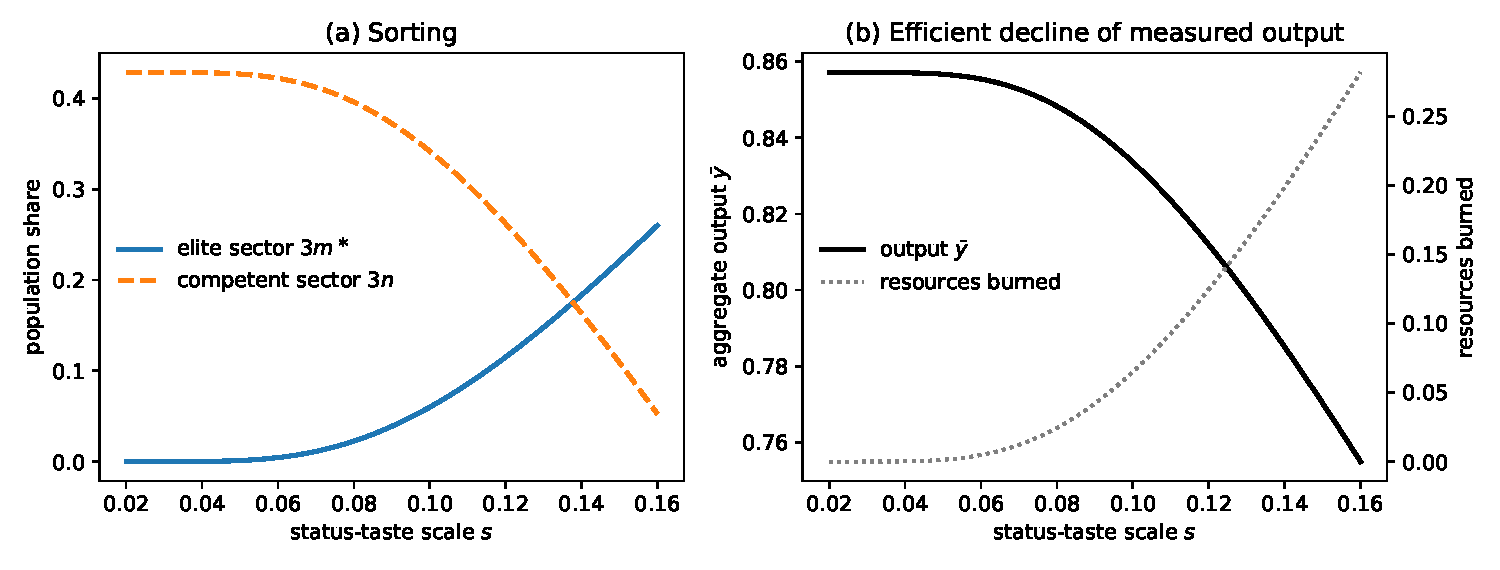
\includegraphics[width=\textwidth]{figures/status_taste_comparative_statics.pdf}
  \caption{Comparative statics in the status-taste scale $s$ ($\eta\sim$
  Exponential, mean $s$). Panel (a): population shares of the elite and competent
  sectors. Panel (b): aggregate output falls and burned resources rise as status
  taste spreads; every equilibrium shown is Pareto optimal
  (Theorem~\ref{thm:nocorrection}). Parameters as in Section~\ref{sec:example}.}
  \label{fig:comparative}
\end{figure}

\section{Positional Status and the Failure of the Welfare Theorem}\label{sec:positional}

Theorem~\ref{thm:nocorrection} rests on status being an \emph{absolute} amenity: the elite-manager membership yields utility $(1+\eta)$ regardless of how many others hold it.
But much of what makes status status is scarcity \citep{hirsch1976social,frank1985demand}: a credential everyone holds confers distinction on no one.
This section makes status positional and shows that everything in Theorem~\ref{thm:nocorrection} breaks --- selectively, and in an instructive way.

\subsection{Positional preferences and equilibrium}

Let $m$ denote the aggregate measure of agents holding an elite-manager seat --- a membership with characteristic $\omega_e$, of which the group set of Section~\ref{sec:model} contains exactly one, $m_{4.1}$ --- and replace the status factor $(1+\eta)$ in the utility specification of Section~\ref{sec:model} with
\begin{equation}\label{eq:positional-utility}
  1 + \eta\, v(m),
\end{equation}
where $v:[0,1]\rightarrow(0,1]$ is continuously differentiable with $v'<0$ throughout and $v(0)=1$: the value of eliteness falls as eliteness spreads.
Each agent is negligible and takes $m$ as given.
(The scalar mass $m$ is unsubscripted; membership labels $m_1,m_{3.1},\dots$ always carry subscripts, so no confusion should arise, and in equilibrium $m$ equals the measure of elite managers, the object the fixed point below denotes $m^\ast$.)
Because utility now depends on \emph{other agents'} memberships, preferences violate the assumptions of \citet{ellickson2006organization}: this is a widespread externality in the sense of \citet{noguchizame2006externalities}.
We accordingly define a \emph{positional group equilibrium} as prices $(p,q)$ and a feasible state $(x,\ell)$ satisfying the three conditions of Section~\ref{sec:framework}, where optimization is with respect to preferences \eqref{eq:positional-utility} evaluated at the aggregate elite mass $m$ induced by the state itself.

Crucially, the externality operates at the level of the \emph{class} of elites (the holders of $m_{4.1}$ across all elite firms) not at the level of any single group.
Membership prices internalize composition effects within a group; they have no instrument that spans groups.
This is precisely the gap in the price system that the welfare theorem needs closed, and it is why the failure below is not a defect of the clubs framework but a fact the framework makes visible.

\subsection{Existence, uniqueness, and self-limiting eliteness}

The wages \eqref{eq:wages}, the output price \eqref{eq:p2}, and the elite-firm break-even income $w_E=z$ are untouched by the externality.
The cutoff condition becomes $(1+\eta^\ast v(m))\,\delta_s\delta_m\, w_E = k$, i.e.,
\begin{equation}\label{eq:positional-cutoff}
  \eta^\ast(m) \;=\; \frac{\eta^\ast_0}{v(m)},
\end{equation}
where $\eta^\ast_0 = \mu k/z - 1$ is the cutoff of Section~\ref{sec:equilibrium}.
Consistency of the conjectured mass with sorting requires $m$ to be a fixed point of
\begin{equation}\label{eq:fixedpoint}
  \rho(m) \;\equiv\; 1 - F\!\left(\frac{\eta^\ast_0}{v(m)}\right).
\end{equation}

\begin{proposition}[Positional equilibrium]\label{prop:positional} Under Assumption~\ref{ass:interior} (maintained at the resulting equilibrium configuration), a positional group equilibrium exists and its elite mass is unique: $\rho$ is continuous and weakly decreasing --- strictly wherever positive --- so $\rho(m)-m$ is strictly decreasing and has exactly one root $m^\ast$, which is strictly positive whenever the support of $F$ extends beyond $\eta^\ast_0/v(0)$.
Moreover: (i) if $m^\ast>0$ then $m^\ast < m_0 \equiv 1-F(\eta^\ast_0)$ --- dilution self-limits the elite; (ii) a FOSD shift of $F$ that is strict at the positional cutoff raises $m^\ast$; if in addition the shift's vertical size at the positional cutoff $\eta^\ast_0/v(m^\ast)$ is weakly smaller than at $\eta^\ast_0$ --- as holds for the exponential scale family used in our examples --- then $m^\ast$ rises by strictly less than $m_0$, so positional concerns dampen the expansion of Proposition~\ref{prop:decline}; (iii) all prices, and the equilibrium values of $p_2$, $w_E$, $n$, and $\bar{y}$ given $m^\ast$, are as in Section~\ref{sec:equilibrium}.
\end{proposition}

The qualification in (ii) is substantive, not decorative: because the positional cutoff $\eta^\ast_0/v(m^\ast)$ exceeds $\eta^\ast_0$, a taste shift concentrated between the two cutoffs would move the positional mass and not the baseline mass, reversing the comparison; damping is a property of shifts that do not favor precisely the diluted region.

Part (i) already delivers a result the baseline cannot: eliteness is self-protecting.
Entry of new elite institutions dilutes the very good they sell, so the market itself polices exclusivity --- no entrant can arbitrage status, because relative position cannot be replicated by replication.

\subsection{Failure of optimality and of core equivalence}

\begin{proposition}[Inefficiency]\label{prop:inefficiency} If $v$ is strictly decreasing, Assumption~\ref{ass:interior} is maintained at the positional equilibrium, and its elite mass is strictly positive, then the positional group equilibrium is not Pareto optimal, and its state does not belong to the core.
\end{proposition}

The proof (Appendix~\ref{app:positional}) is constructive and exploits the equilibrium's own structure.
Every non-elite agent (laborers, competent managers, leisure-takers) is at reservation utility and indifferent among their activities; so is every marginal elite.
The planner therefore shuts a small mass $dm$ of elite triples and opens competent triples in the ratio that restores material balance in both goods --- a reallocation that is \emph{exactly} feasible because both adjustment directions have zero value at equilibrium prices.
The released laborers and the redeployed leisure-takers are indifferent; the shut firms' managers lose only their near-marginal status surplus, an amount vanishing relative to $dm$ that the remaining elites' first-order de-dilution gain strictly covers through explicit compensation.
But $v(m)$ rises, so every inframarginal elite is strictly better off: a Pareto improvement, executable by the grand coalition, so the state is blocked and core equivalence fails.
The contrast with Theorem~\ref{thm:nocorrection} is exact: there, shutting elite firms had to take status away from people who had paid its price; here, shrinking the elite \emph{creates} status out of scarcity.

\subsection{Over-entry and the membership tax}

At the laissez-faire equilibrium the marginal entrant weighs the private value of elite membership against its price, but ignores the dilution imposed on every inframarginal elite.
The planner's cutoff condition (Appendix~\ref{app:positional}) equates the marginal type's surplus to the aggregate dilution wedge
\begin{equation}\label{eq:wedge}
  t^\ast \;=\; \left|v'(m^\ast)\right|\, \frac{w_E}{\,1+\eta^\ast v(m^\ast)\,}
  \int_{\eta\geq\eta^\ast}\!\! \eta\, dF(\eta),
\end{equation}
expressed in units of the marginal entrant's income.
Since the equilibrium sets the marginal surplus to zero while the wedge is strictly positive, there is over-entry.

\begin{proposition}[Membership tax]\label{prop:tax} Let a tax $t$ be levied on the elite-manager membership, with revenue rebated as a uniform lump sum.
(i) At any fixed rebate level, the fixed-point map remains continuous and weakly decreasing in the elite mass, strictly wherever positive, so the equilibrium elite mass is unique given the rebate and is strictly decreasing in $t$ while positive.
(ii) The laissez-faire equilibrium exhibits over-entry: its cutoff sets the marginal entrant's surplus to zero, whereas every Pareto-optimal cutoff allocation requires that surplus to equal the strictly positive wedge \eqref{eq:wedge}.
(iii) At $t=0^{+}$, the output response decomposes into three channels, $d\bar{y}/dt = \bar{y}_m\,m'(0^{+}) + \bar{y}_T\,m^\ast + \bar{y}_t$: a de-entry term, in which $\bar{y}_m$ is the derivative of Proposition~\ref{prop:decline} (negative under condition \eqref{eq:decline}, so that with $m'(0^{+})<0$ the term is positive); a rebate term $\bar{y}_T\,m^\ast<0$, operating through reservation incomes and the output price; and a direct incidence term $\bar{y}_t = \phi m^\ast/[2c+2r+(\mu+2\lambda-3)k]>0$, the tax's reduction of elite consumption demand releasing resources to production; output rises if and only if the two positive channels together dominate the rebate term.
\end{proposition}

The propositions state what is proven; the numerical continuation below shows that their hypotheses are not vacuous.
Part (iii) deserves emphasis because it reverses the baseline's policy content.
Under absolute status, taxing the elite sector reduces welfare (it undoes priced, efficient consumption).
Under positional status the tax raises welfare in the example, and it raises output whenever the de-entry and incidence channels together dominate the rebate's price effect; when both margins improve, as they do in the example, there is no equity--efficiency trade-off: the taxed activity was destroying value at the margin in both senses.
Dominance is a genuine condition rather than a formality; a taste distribution thin at the cutoff makes entry unresponsive, and the rebate's price effect can then reverse the output gain even as the elite mass falls.
In the example the three channels are $+0.0160$, $-0.0063$, and $+0.0037$, a total of $+0.0134$, so both margins improve (Appendix~\ref{app:positional}).
The practical diagnostic offered by the theory is thus a question about preferences, not about waste: \emph{is elite status valued in itself, or valued because others lack it?}
Only in the second case is there anything for policy to correct.

\subsection{Numerical continuation}

Continuing the example of Section~\ref{sec:example} with $v(m)=1/(1+\kappa m)$, $\kappa=25$: the elite mass falls from $m_0\approx 0.0200$ to $m^\ast\approx 0.0086$, with $v(m^\ast)\approx 0.82$, so dilution cuts the elite by more than half, and output rises to $\bar{y}\approx 0.847$.
The same FOSD taste shift (the exponential mean rising from $s=0.10$ to $0.11$) that raises the baseline elite mass by $0.0085$ raises the positional mass by only $0.0023$.
Utilitarian welfare is strictly increasing in the membership tax at $t=0$; the welfare-maximizing tax in the example is $t^{W}\approx 0.31$ (about $5.4\%$ of the elite manager's net income, and close to the first-order Pigouvian level $t^\ast\approx 0.35$), under which the elite mass falls to $0.0050$ and output rises further.
Figure~\ref{fig:positional} displays the fixed point and the welfare curve.
All computations are verified in \texttt{analysis/positional\_model.py}.

\begin{figure}[t]
  \centering
  
\includegraphics[width=\textwidth]{figures/positional_tax.pdf}
  \caption{The positional equilibrium. Panel (a): the map $\rho$ of
  \eqref{eq:fixedpoint} is strictly decreasing, giving a unique elite mass
  $m^\ast$, strictly below the non-positional mass $m_0$ (dotted). Panel (b):
  utilitarian welfare as a function of the membership tax $t$ (uniform lump-sum
  rebate); welfare rises for all small taxes --- the signature of over-entry ---
  and peaks at $t^{W}$. Parameters as in Section~\ref{sec:example} with
  $v(m)=1/(1+25m)$.}
  \label{fig:positional}
\end{figure}

\section{Dynamics: Bequests, Growth, and Rational Impoverishment}\label{sec:dynamics}

The static analysis holds wealth fixed.
This section lets the economy accumulate: each generation inherits the resources its parents saved, plays the club economy of Sections~\ref{sec:model}--\ref{sec:positional} within its lifetime, and bequeaths.
Three questions organize the analysis.
Does the market for elite status expand or contract as an economy grows?
Does the elite sector's resource burn feed back into accumulation?
And, the question any reader of Section~\ref{sec:equilibrium} will ask, if status spending erodes the wealth of future generations, do rational, forward-looking agents really let it happen?

\subsection{The overlapping-generations economy}

Time is discrete, $t=0,1,2,\dots$.
Each period a measure-one generation is born, inherits per-capita resources $k_t$ (the input good), and lives for one productive period within which the schooling-then-employment sequence of the static model unfolds (memberships are dated within the period, as in \citealt{ellickson2006organization}).
Preferences extend \eqref{eq:utility} with a warm-glow bequest made in the \emph{produced} good --- output invested today is the resource base of the next generation:
\begin{equation}\label{eq:olg-utility}
  u \;=\; d(\ell;\eta)\; x_1^{\zeta/2}\, x_2^{\zeta/2}\, b^{\,1-\zeta},
  \qquad \zeta\in(0,1),
\end{equation}
so an agent with net income $w$ spends $(\zeta/2)w$ on each consumption good and $(1-\zeta)w$ on the bequest, and attains indirect utility $d\,w\,\psi(p_2)$, where $\psi(p_2)$ is a price index common to all agents (Lemma~\ref{lem:period}) --- \emph{still linear in net income}.
Every occupational-indifference condition, membership price, the output price \eqref{eq:p2}, the cutoff \eqref{eq:etastar}, and the positional fixed point \eqref{eq:fixedpoint} therefore carry over verbatim at wealth $k_t$; only the competent-sector scale $n$ adjusts for the saving margin, and $\zeta=1$ recovers the static model exactly (Lemma~\ref{lem:period} in Appendix~\ref{app:dynamics}).
Invested output converts into next-period resources at a rate $\theta>0$ (a constant-returns storage activity, freely operated, whose linearity makes it profitless and ownerless; the input good itself perishes at the period's end), and children inherit the economy-wide average bequest:
\begin{equation}\label{eq:transition}
  k_{t+1} \;=\; \xi(k_t) \;\equiv\; \theta\,(1-\zeta)\,\frac{\bar{w}(k_t)}{p_2(k_t)},
\end{equation}
where $\bar{w}(k)$ is aggregate net income --- endowment plus the value added of the schools and firms that form at wealth $k$.
Uniform inheritance abstracts from within-generation heterogeneity in inheritances (the gift is pooled, so there are no dynasties in the model, only generations); the Galor--Zeira-style interaction of inherited inequality with elite membership is an important extension we defer.

\begin{definition}\label{def:dynamiceq}
Given $k_0>0$, a \emph{dynamic equilibrium} is a sequence of period allocations and prices such that, in every period $t$: the allocation is a group equilibrium of the period economy at wealth $k_t$, namely the interior equilibrium of Lemma~\ref{lem:characterization} (or its positional counterpart) when Assumption~\ref{ass:interior} holds at $k_t$, and the elite-free equilibrium when $z(k_t)\leq 0$; and $k_{t+1}$ is given by \eqref{eq:transition}.
(Outside these two cases the dynamic equilibrium is undefined; the domain $K$ of Proposition~\ref{prop:map} excludes them.)
\end{definition}

Because preferences \eqref{eq:olg-utility} contain no forward-looking argument, the definition is genuinely recursive: no agent's optimization requires forecasting, and each period's prices depend only on $k_t$.

\begin{proposition}[The transition map]\label{prop:map} Let $K\subset\R_+$ be an interval on which the period equilibrium of Definition~\ref{def:dynamiceq} is well defined (Assumption~\ref{ass:interior} where the elite sector is viable, the elite-free interior configuration elsewhere).
Under \eqref{eq:olg-utility} and condition \eqref{eq:decline}, so that the elite sector is inactive near the origin: (i) the within-period allocation at wealth $k_t\in K$ is the club equilibrium of Section~\ref{sec:equilibrium} (or Section~\ref{sec:positional}) at $k_t$; (ii) $\xi$ is continuous on $K$, with $\xi'(0^+)=\theta(1-\zeta)\phi/(c+r)$, and the elite-free map is bounded (diminishing returns operate through the price of investment, $p_2(k)$, which rises with wealth); (iii) if $\theta(1-\zeta)\phi>c+r$, the origin repels, and any interior crossing of the diagonal from above is a steady state, stable whenever $|\xi'|<1$ there.
\end{proposition}

In our parameterization $K$ comfortably contains the steady states and transition paths studied below, each crossing is unique with $|\xi'|<1$, and at substantially higher wealth or taste the interior configuration eventually fails (the competent sector's market-clearing scale reaches zero, and at extreme wealth every agent demands the elite path), at which point the map would have to be extended by the corner regimes, which we do not need.
The recursivity of Definition~\ref{def:dynamiceq} answers the ``do they really let it happen?'' question in its sharpest form: not only are expectations correct along the path --- they are not even required.
The path $(k_t)$ generated by \eqref{eq:transition} is common knowledge, and every generation can compute the decline it participates in.
No individual would behave differently with perfect foresight: each is atomistic, her gift cannot move the aggregate, and her within-period choices are optimal at the prices she faces.
The impoverishment we exhibit below is not a mistake, a bubble, or a failure of anticipation; it is what optimizing behavior looks like when status is among the things people want.
We are careful about what this does and does not establish: with warm-glow preferences the absence of an expectational channel is a feature of the specification.
Appendix~\ref{app:motive} shows that the feature is not load-bearing.
The paper's status margin (prices, wages, the cutoff, and the elite mass at every wealth level) is invariant to the transfer motive within the degree-one preference class: any common savings rule, forward-looking or not, changes only the volume of saving and hence the speed and destination of the wealth path, never the within-period mechanism (Proposition~\ref{prop:invariance}).
And warm glow is not an evasion but a minimal requirement: under pooled inheritance, purely altruistic parents free-ride completely and transfer nothing (Proposition~\ref{prop:commons}), so some direct gift motive is necessary for the economy to persist at all.
The natural sharpening, dynasty-specific transfers with forward-looking parents, is discussed in Section~\ref{sec:discussion}.

\subsection{Status is a luxury}

\begin{proposition}[Luxury]\label{prop:luxury} The elite cutoff $\eta^\ast_0(k)=\mu k/z(k)-1$ is strictly decreasing in $k$ --- and hence the elite mass $m^\ast(k)$ strictly increasing in $k$ wherever the cutoff is interior to the support of $F$ --- if and only if $\alpha(c+r) < \beta c + \tau r$: precisely the resource-productivity condition \eqref{eq:decline} of Proposition~\ref{prop:decline}.
\end{proposition}

The mechanism is instructive.
The elite sector's excess costs --- the school's burn $(\tau-1)r$, the firm's burn $(\beta-1)c$ --- are \emph{fixed} resource costs, while every wage in the economy scales with wealth.
As $k$ grows, the burn shrinks relative to the status discount that finances it, so the marginal entrant needs less taste for status to justify entry: rich societies buy more eliteness not because their preferences differ but because they can better afford the waste.
Below a viability threshold ($z(k)\leq 0$) the elite sector cannot break even at any taste level: in this economy of identical endowments, a society too poor to cover the burn has no market for wasteful status.
(With endowment inequality, a wealthy stratum can sustain such a market at low \emph{average} wealth --- historical markets in offices, commissions, and titles are the obvious examples --- so the proposition is a within-economy comparative static on aggregate wealth holding the distribution fixed.)
No nonhomotheticity is assumed in \emph{preferences}; the luxury property is technological, produced by fixed real resource requirements meeting wages that scale with wealth, and it would attenuate if the elite sector's costs scaled with wealth as well --- an empirical question about the cost structure of elite institutions.
That the operative condition is the same one that makes the elite sector a drag on output is what disciplines the mechanism.

\subsection{The status drag and the spread of taste}

\begin{proposition}[Status drag]\label{prop:drag} At any wealth $k$ at which the elite sector is active, $\operatorname{sign}\,\partial \xi/\partial m^\ast = \operatorname{sign} [\alpha(c+r)-(\beta c+\tau r)]$.
Under condition \eqref{eq:decline}, therefore: (i) the transition map lies strictly below the no-elite-sector map wherever the elite is active, so that whenever each map crosses the diagonal once in that region, the steady states are ordered $k^\ast_{\mathrm{elite}} < k^\ast_{\mathrm{none}}$; (ii) a FOSD spread of the status-taste distribution, strict at the relevant cutoffs, lowers $\xi$ pointwise (strictly where the elite is active), and under the same single-crossing proviso strictly lowers the steady state; (iii) under positional status, and for taste shifts satisfying the damping hypothesis of Proposition~\ref{prop:positional}(ii) at the cutoffs corresponding to each wealth level, the pointwise decline of $\xi$ is strictly smaller wherever the elite sector is active.
\end{proposition}

One condition (the elite sector produces less output per unit of resources) now governs all three of the paper's mechanisms: the static output decline (Proposition~\ref{prop:decline}), the luxury property (Proposition~\ref{prop:luxury}), and the dynamic drag (Proposition~\ref{prop:drag}).
In the example every proviso holds, and the three steady states order as the propositions suggest: $k^\ast_{\mathrm{abs}} < k^\ast_{\mathrm{pos}} < k^\ast_{\mathrm{none}}$.
Together they compose the paper's dynamic narrative: growth makes status affordable, status absorbs the resources that fund growth, and the economy converges to a steady state with permanently lower wealth than its status-free counterfactual --- with every generation optimizing, and every generation aware.

Two features of the dynamics deserve emphasis.
First, there is no collapse: since the elite sector is unviable at low wealth (Proposition~\ref{prop:luxury}), the map near the origin is elite-free and the origin repels (Proposition~\ref{prop:map}).
Status spending impoverishes; it does not extinguish.
The ``self-destruction of the economy'' takes the form of a permanently lower steady state, not a death spiral --- and the mechanism that limits the damage is the same one that creates it: as wealth falls, the economy can no longer afford its elite.
Second, positional dilution is again protective, now dynamically: because entry dilutes status, the elite mass responds far less to spreading taste, and steady-state wealth barely moves.
Societies in which status is relative are (by that very relativity) partially immunized against the status drag.

On intertemporal welfare we claim less, deliberately.
Within each period, the absolute-status allocation is Pareto optimal given $k_t$ (Theorem~\ref{thm:nocorrection}); but future generations are not parties to any period's core, warm-glow bequests \citep{andreoni1990} internalize the intergenerational margin only partially, and overlapping-generations economies admit dynamic inefficiency of the \citet{diamond1965} type.
We emphasize accordingly that the steady-state comparisons above are statements about \emph{wealth}, not welfare: if the warm-glow path overaccumulates, a lower steady state need not be a worse one.
Whether the equilibrium path is efficient among feasible paths --- and by what criterion, given that the glow itself is a utility flow --- is a question we flag for the sequel rather than resolve here.

\subsection{Numerical continuation}

Continuing the running example with $\zeta=0.8$ (a 20\% bequest share) and $\theta$ calibrated so that the absolute-status steady state is exactly the static example's wealth, $k^\ast=2$: the steady state is stable ($\xi'(k^\ast)=0.17$), with the static example's prices, wages, cutoff, and elite mass reproduced as the steady-state allocation.
The no-elite counterfactual steady state is $2.085$; the positional steady state $2.045$.
As the taste scale rises from $s=0.10$ to $s=0.19$, the absolute-status steady state falls to $1.73$ --- a 16.8\% wealth loss relative to the no-elite benchmark, with the elite sector (managers together with their firms' workers) swelling to about a fifth of the population, while the positional steady state falls only to $1.97$ (a 5.7\% loss).
After a taste shift to $s=0.18$, the transition $2.00\rightarrow1.74\rightarrow1.77\rightarrow1.76$ settles within three generations; the mild oscillation reflects the map's locally negative slope at the new steady state ($\xi'\approx-0.08$): a higher inherited $k$ supports a larger elite, which shrinks the aggregate gift --- the luxury mechanism operating period by period.
Figure~\ref{fig:dynamics} displays the maps and the steady-state decline.
All computations are verified in \texttt{analysis/dynamic\_model.py}.

\begin{figure}[t]
  \centering
  
\includegraphics[width=\textwidth]{figures/dynamics_collapse.pdf}
  \caption{Dynamics. Panel (a): transition maps at baseline taste ($s=0.1$) for
  the no-elite counterfactual and the absolute-status economy, and the
  absolute-status map after a taste spread ($s=0.18$); the marked point is the
  calibrated steady state $k^\ast=2$. Panel (b): stable steady-state wealth as
  the taste scale $s$ rises --- the absolute-status economy is impoverished by
  the spread of status taste, the positional economy is largely protected by
  dilution. Parameters as in Sections~\ref{sec:example}
  and~\ref{sec:positional} with $\zeta=0.8$, $\theta=5.141$.}
  \label{fig:dynamics}
\end{figure}

\section{Empirical Content}\label{sec:empirics}

The model was built to explain a pattern, and it returns a set of predictions sharp enough to be wrong.
We collect them here, together with the existing evidence that bears on each.

\textbf{Compensation.}
Corollary~\ref{cor:wages} reproduces the configuration of conspicuous gross salaries alongside a predicted (not yet measured) inferior net position, and its comparative statics are sharper than the accounting identity suggests.
Because the elite wage is pinned by the firm's revenue, a change in elite tuition is absorbed \emph{one for one by the status discount}: the equilibrium gross wage satisfies $-q_{4.1}=\alpha p_2\phi-\beta c+(3-2\lambda^e)k-k$, in which $\tau$ does not appear (machine-verified).
The model therefore predicts \emph{zero incidence of elite tuition on elite salaries} --- where a competitive human-capital account, in which wages must recoup education costs on the margin, predicts positive pass-through.
Tuition-shock episodes in credential markets where students pay the full posted price, so that tuition changes are borne by the student rather than offset by aid (elite professional degrees rather than subsidized undergraduate education), are thus a discriminating experiment against cost-recoupment accounts; the design requires elite-specific shocks differenced against the non-elite track, since a common school-cost shock passes through at rate $\alpha$ in this very model.
An entry-rationed human-capital account with wages pinned by marginal product would also deliver zero pass-through, so it is the joint prediction, zero tuition incidence together with the inferior net position below, that isolates the status mechanism.
The second prediction is the net one: returns to the elite career track computed net of the full cost of elite education should fall below the non-elite track's --- a claim no current estimate supports or refutes, and one the best causal evidence pressures: admission effects large enough to move mean earnings \citep{chettydemingfriedman2026} and top-percentile odds \citep{zimmerman2019elite} exceed any plausible tuition differential, which through the lens of the identity says observed premia carry scarcity rents (and, in observational comparisons, bundled ability) on top of the status-financed component.
The decomposition then bounds the status component; it does not cap the premium.

\textbf{Firm accounts versus resource accounts.}
In the central configuration, output, revenue, and pay comparisons all flatter the elite sector, and with $\alpha\geq\beta$ (as in our example) productivity comparisons do as well.
The drain appears nowhere on any firm's books, because it is incurred in the school system (Proposition~\ref{prop:decline}); and it need not appear as a fall in measured GDP either, since national accounts value education output at input cost, so the burn is booked as education-sector value added.
The model-consistent observable is therefore not aggregate TFP but \emph{credentialing resources per managerial position filled, economy-wide}: $(nr+m^\ast\tau r)/(n+m^\ast)$ in the model's notation.
The cost per elite slot, $\tau r$, is a technology constant; the economy-wide average rises purely through composition, as the expensive credential claims a growing share of positions, and the model predicts it rises with wealth and with the spread of status taste while firm-level performance metrics improve (machine-verified: from $1.0$ to $3.5$ across the example's taste scan).
Credential inflation (more resources devoted to obtaining a given position) is this wedge in labor-market form, and it is measurable where TFP decompositions are not.
We note the magnitude honestly: elite credentialing is a small share of aggregate resources in any modern economy, so the mechanism's aggregate bite in our stylized examples (double-digit steady-state losses) reflects the model's deliberately outsized elite sector, not a calibration.

\textbf{Status as a luxury.}
Proposition~\ref{prop:luxury} predicts that the elite share of the population rises with aggregate wealth, holding tastes and the endowment distribution fixed.
The prediction is a within-economy comparative static, not a cross-country ranking: because our agents share a common endowment, the model's ``poor economy'' is one in which \emph{no one} can cover the burn, whereas historically poor societies with wealthy strata ran flourishing markets in skill-free position (venal offices, purchased commissions, sold degrees) exactly as an endowment-heterogeneous version would predict.
The mechanism the proposition isolates --- a fixed resource burn financed by wages that scale with wealth --- implies that within an economy, growth expands the elite share, and ties that expansion to the same condition that governs the aggregate drag.

\textbf{Distinguishing absolute from positional status.}
The paper's two welfare regimes are observationally similar in a cross-section (wasteful elite institutions persist in both) but differ in their dynamics.
In the positional equilibrium all monetary prices coincide with the absolute-status benchmark (Proposition~\ref{prop:positional}(iii)); dilution operates through quantities, not wages, so the discriminating observable is the elasticity of the elite share to demand shifts.
Positional status implies damped responses, for shifts satisfying the damping hypothesis of Proposition~\ref{prop:positional}(ii), because each entrant erodes the prize; absolute status implies the full one-for-one quantity response.
Historical episodes shifting the demand for elite positions therefore identify the operative regime, provided the shift itself is measured, and with it the policy conclusion, since only the positional regime admits a welfare-improving membership tax (Proposition~\ref{prop:tax}).

\textbf{What the causal evidence can and cannot say.}
The best-identified estimates of elite-education effects compare admitted with rejected applicants and find gains concentrated in top-tail outcomes and access to prestigious positions, large enough to move mean earnings \citep{zimmerman2019elite,chettydemingfriedman2026}.
Such designs identify \emph{relative} effects and cannot distinguish the creation of output from the reallocation of positions.
The model delivers precisely this coexistence: admission carries positive private returns, in status utility and in gross pay up to excess tuition, while the aggregate return to elite-sector expansion is zero or negative, because the burn sits on the school system's books rather than any firm's.
The magnitude gap between the model's bounded premia and the estimated effects is carried by the scarcity rents discussed above; and the features a relative-effects design cannot rule out in the data-generating world (a fixed stock of top positions, purely positional gains) are exactly the ones such designs cannot distinguish from output creation.
The aggregate margin, not the individual one, is where the model's distinctive content lies.

\textbf{Magnitudes.}
The examples above are built to display mechanisms, not to measure them; this final block asks what the mechanism could plausibly amount to in aggregate, and answers with a bound.
The model supplies the required mapping exactly.
At the steady states of Section~\ref{sec:dynamics}, the wealth gap between the elite-active economy and its status-free counterfactual satisfies the closed-form identity (Remark~\ref{rem:loss} in Appendix~\ref{app:dynamics})
\[
\frac{k^\ast_{\mathrm{none}}-k^\ast_{\mathrm{elite}}}{k^\ast_{\mathrm{none}}} \;=\; M\cdot b,
\]
where $b$ is the share of steady-state resources burned by elite credentialing and the multiplier $M$, given in closed form in the remark, contains no taste parameter: the entire taste distribution enters the loss only through the observable burn share.
In the running example $M=1.25$.
On the empirical side, U.S.\ degree-granting postsecondary institutions spent \$702 billion in 2020--21 \citep{nces2023expenses}, roughly three percent of GDP \citep{bea2022gdp}, and the elite segment of that spending is small: fewer than half of one percent of Americans attend the twelve Ivy-Plus colleges \citep{chettydemingfriedman2026}.
Suppose, deliberately extremely, that the status-intensive segment enrolls five percent of students (an order of magnitude beyond Ivy-Plus scale, room enough for every elite private and flagship professional program), that it spends four times the national average per student, and that \emph{all} of that spending is burn rather than skill production --- the polar case of Remark~\ref{rem:polar} applied to the entire segment.
Then $b$ is at most twenty percent of three percent, or $0.6$ percent of resources, and the implied steady-state wealth loss, at the example's multiplier, is about three-quarters of one percent.
A central attribution --- a segment at one percent of enrollment, with only its spending premium over the national average, taken as one times that average, counted as burn --- puts the loss at a few hundredths of a percent.
(All arithmetic is machine-verified in \texttt{analysis/magnitude\_bound.py}.)
The conclusion is deliberately modest, and we state it plainly: this mechanism does not explain aggregate stagnation.
Its aggregate bite scales with the resources the status sector absorbs, and those are small.
What the theory changes is the interpretation of institution-level facts --- who finances elite waste, why firm accounts cannot reveal it, which observables track it, and when policy has anything to correct --- and for the participants the distributional stakes of Corollary~\ref{cor:wages} are first-order regardless of $b$.
Two scope notes bound the bound itself.
It prices the burn of formal credentialing, so if positional competition operates through channels the education accounts do not book (grooming, screening, tournament hours), the relevant $b$ exceeds the credentialing envelope.
And it is a statement about the steady-state wealth of the model economy under uniform inheritance, not a growth-accounting decomposition for any actual one.

\section{Discussion}\label{sec:discussion}

\textbf{GDP versus welfare.}
Propositions~\ref{prop:coexist}--\ref{prop:decline} and Theorem~\ref{thm:nocorrection} jointly formalize a distinction the public debate conflates: what declines as elite status spreads is real output net of resources burned, a quantity that neither firm accounts nor standard national accounts isolate, and not what agents maximize.
Any diagnosis of ``inefficiency'' from output or TFP data alone presumes status utility does not count --- a normative stance that should be argued, not assumed.

\textbf{Positional scarcity and rents.}
Positional status supplies a natural amplification channel for observed premia: with $v$ strictly decreasing, the elite characteristic is in endogenously limited supply, and extensions in which firms compete for a capped pool of incumbent elites would shift $q_{4.1}$ further toward scarcity rents (widening observed premia beyond tuition reimbursement) without disturbing the marginal entrant's status discount.

\textbf{Extensions.}
Three extensions strike us as most valuable.
First, dynasty-specific inheritance: uniform inheritance isolates the aggregate mechanism, but letting parents bequeath directly to their children would interact inheritance with elite membership in the manner of \citet{galorzeira1993}, and would let the model speak to intergenerational mobility at the top.
The sign is worth stating honestly: because elite managers accept lower \emph{net} incomes, dynasty-specific bequests would transmit less wealth down elite lines --- the status discount is dynastically self-impoverishing --- so the model's persistence is institutional rather than dynastic, and reconciling the two is precisely what the extension is for.
Relatedly, replacing warm glow with forward-looking altruism would make the rationality of decline a theorem about expectations rather than a feature of the specification; under pooled inheritance, altruistic parents face a commons in the aggregate gift, which plausibly strengthens the drag, though we have not proven this.
Second, parents who value their children's \emph{status} rather than the bequest itself --- the natural sharpening of the warm-glow specification, which would make elite membership itself heritable in demand.
Third, intertemporal welfare: each period's absolute-status allocation is optimal given its inheritance, but the path's efficiency across generations --- and what, if anything, a generation-spanning planner could improve even in the absolute-status world --- is open, and the answer plausibly differs between the absolute and positional regimes.

\section{Conclusion}\label{sec:conclusion}

Elite institutions that consume more than they return are not an affront to the theory of competitive markets; they are an application of it.
When status is a priced membership, competition sustains the institutions that produce it for the same reason it sustains any other industry: willing buyers cover the costs.
Competition remains exacting about the products markets actually trade: a status-equivalent technology at lower resource cost would displace these institutions in every equilibrium (Theorem~\ref{thm:displacement}); what survives is dominated only in the material projection of its product.
This paper has priced elite status explicitly, in the most demanding competitive framework available, and traced the consequences through displacement, compensation, output, welfare, and accumulation.
The results discipline both sides of a familiar argument.
Against the presumption that visible elite premia and superior elite-firm performance certify productive efficiency, the model shows both arising in an economy converging to permanently lower material wealth.
Against the presumption that elite waste is a market failure demanding correction, the model shows the waste is Pareto optimal --- unless status is valued for its scarcity, in which case, and within the environments we model only in that case, there is over-entry, which a corrective membership tax can convert into gains in output and welfare together, as in our example.
The operative empirical question is therefore not whether elite institutions are wasteful, but why their members want them: for what membership is, or for what it is not shared with.
Markets work either way; material efficiency follows in neither.

\appendix

\section{Derivations and Proofs}\label{app:derivations}

All computations in this appendix are verified symbolically in \texttt{analysis/static\_model.py}.

\subsection{Demand and indirect utility}
An agent with net income $w$ solves $\max_{x_1,x_2} d\sqrt{x_1x_2}$ subject to $x_1+p_2x_2=w$, giving $x_1=w/2$, $x_2=w/(2p_2)$, and indirect utility $d\,w/(2\sqrt{p_2})$.

\subsection{Dominated lists}
\begin{lemma}\label{lem:dominated} At any prices satisfying \eqref{eq:prices} with $r,\tau r>0$, every feasible list other than the five in Section~\ref{sec:model} is strictly dominated.
\end{lemma}

\begin{proof}
The consumption sets allow at most one school and at most one job, and a graduate of one school type cannot hold the other type's managerial membership, so the only feasible lists beyond the five are schooling with no job and schooling combined with a laborer job.
(i) Schooling with no job yields taste factor $d\leq\delta_s<1$ and net income $k-q_j<k$, dominated by leisure.
(ii) Schooling plus a laborer job multiplies the laborer's taste factor by $\delta_s<1$ and subtracts tuition, dominated by the same laborer job alone.
\end{proof}

\subsection{Proof of Lemma~\ref{lem:characterization}}
\emph{Budget balance.}
Schools: $q_1-r=0$, $q_2-\tau r=0$ by \eqref{eq:prices}.
Competent firms: $q_{3.1}+2q_{3.2} - c + p_2\phi = (k-r-\mu k) + 2(k-\lambda k) - c + p_2\phi = 0$ by \eqref{eq:p2}.
Elite firms: $q_{4.1}+2q_{4.2} - \beta c + p_2\alpha\phi = 0$ reduces, using \eqref{eq:p2}, to $w_E = z$, which is \eqref{eq:etastar}.
\emph{Optimization.}
By Lemma~\ref{lem:dominated} only the five vocational choices need comparison; by construction of \eqref{eq:wages} and \eqref{eq:cutoff}, types below $\eta^\ast$ are indifferent among the four non-elite choices and strictly prefer them to the elite path, types above strictly prefer the elite path, and the marginal type is indifferent.
\emph{Consistency and material balance.}
The stated measures fill every group type in the required proportions; market clearing \eqref{eq:clearing} solves
\begin{equation}\label{eq:nclosed}
  n \;=\; \frac{k - (1-3m^\ast)\frac{k}{2} - m^\ast\left[\frac{w_E}{2} +
  w_{L^\ast} + \tau r + \beta c\right]}
  {\frac{w_M}{2} + w_L - \frac{3k}{2} + r + c},
\end{equation}
positive under Assumption~\ref{ass:interior}.
\emph{Walras.}
Substituting \eqref{eq:nclosed} and \eqref{eq:etastar} into the $y_2$ market, demand $\sum \text{(measures)}\times w/(2p_2)$ equals supply $\phi(n+\alpha m^\ast)$ identically (machine-verified).
Uniqueness of the interior configuration follows because, when a positive measure of agents also holds the empty list, indifference with leisure and budget balance imply \eqref{eq:wages}--\eqref{eq:etastar}, and \eqref{eq:nclosed} is linear in $n$.
\qed

\subsection{Proof of Proposition~\ref{prop:coexist}} Subtracting the two firm budget-balance conditions, $p_2\phi(1-\alpha) = (w_M - w_E) - 2(w_{L^\ast}-w_L) - (\beta-1)c - (\tau-1)r$ after substituting \eqref{eq:prices}; the left side is positive iff $\alpha<1$, given $p_2>0$.
\qed

\subsection{Proof of Proposition~\ref{prop:decline}} $\eta^\ast$ solves \eqref{eq:etastar}, which contains no object depending on $F$; a FOSD shift weakly raises $1-F(\eta)$ pointwise, and strictness at $\eta^\ast$ raises $m^\ast=1-F(\eta^\ast)$ strictly.
Differentiating $\bar{y} = \phi(n+\alpha m^\ast)$ with $n$ from \eqref{eq:nclosed}, \[ \frac{d\bar{y}}{dm^\ast} \;=\; \phi\left(\alpha - 1 + \frac{d(n+m^\ast)}{dm^\ast}\right),
\qquad
\operatorname{sign}\frac{d\bar{y}}{dm^\ast} = \operatorname{sign}\big[\alpha(c+r) - (\beta c + \tau r)\big], \] where the second equality is by direct computation (machine-verified in \texttt{analysis/static\_model.py}): $\frac{d\bar{y}}{dm^\ast} \;=\; \frac{\phi\,[\alpha(c+r)-(\beta c+\tau r)]}{2c+2r+(\mu+2\lambda-3)k},$ whose denominator is positive.
\qed

\section{Verification of Framework Assumptions}\label{app:assumptions}

\emph{Consumption sets.}
$X_a = \R^2_+\times\Lists_a$ with $\Lists_a$ the lists satisfying the schooling prerequisites and the at-most-one-school, at-most-one-job bounds; the list bound is $\bar\ell=2$.
Free upward disposal in private goods holds.
The correspondence $a\mapsto X_a$ is constant in $a$ (types differ only through $u$), hence measurable.

\emph{Utility.}
$u(x,\ell;\eta)$ is continuous, strictly increasing in $x$ on the interior of $\R^2_+$ for each $\ell$, and jointly measurable since $\eta\mapsto d(\ell;\eta)$ is continuous and $a\mapsto\eta_a$ measurable.
One boundary caveat deserves note: $h=\sqrt{x_1x_2}$ is constant along the axes, so the strict-monotonicity assumption of \citet{ellickson2006organization} fails there; their arguments use monotonicity only through local nonsatiation and budget exhaustion, which $u$ satisfies everywhere on $\R^2_+$, so the invocation of their Theorem~1 is unaffected.

\emph{Desirable endowments.}
$u_a(e_a,0) = h(k,0) = 0$.
If $u_a(x,\ell)>0$ then $x\gg 0$, so any reduction $x'\leq x$, $x'\neq x$, remains in $X_a$ (consumption sets impose no lower bound above zero); hence endowments are desirable in the sense of \citet[Section~9.4]{ellickson2006organization}, and their Theorem~1 delivers membership of every equilibrium state in the strong core and strong Pareto optimality.

\emph{Existence.}
Not invoked: Lemma~\ref{lem:characterization} exhibits equilibrium in closed form.
(For non-interior parameter configurations, existence follows from Theorem~2 of \citealt{ellickson2006organization} upon verifying group irreducibility; this is routine but omitted until needed.)

\section{Displacement: Proofs}\label{app:displacement}

The openness computations of part (ii) are verified in \texttt{analysis/displacement\_theorem.py}.

\subsection{Part (i), core route}
Let $(x,\ell)$ be feasible with $\nu(g)>0$, and let $S$ be the assumed positive-measure set of agents consuming strictly positive bundles.
We exhibit a strong block by the grand coalition.
Assign to every agent the list $\hat\ell_a=\ell_a[g\rightarrow g']$; clause (E1) preserves individual feasibility, and the substitution preserves list lengths, so the bound $\bar\ell$ is respected.
Consistency holds because the seats released from type-$g$ groups fill type-$g'$ groups in exactly the required proportions (the profiles coincide): $\hat\nu(g')=\nu(g')+\nu(g)$, $\hat\nu(g)=0$, and all other masses are unchanged.
Aggregate net output changes by $\nu(g)(y'-y)\geq 0$, $\neq 0$; choose a good $j$ with $y'_j>y_j$ and distribute the released surplus $\nu(g)(y'_j-y_j)>0$ of good $j$ uniformly across agents, which free upward disposal keeps inside every consumption set.
By (E2) the substitution leaves every agent's utility unchanged, the added goods leave almost every agent weakly better off, and every agent in $S$ is strictly better off, utility being strictly increasing at interior bundles.
This is a strong block: the state is not in the strong core.
Endowments being desirable (Appendix~\ref{app:assumptions}), every group-equilibrium state belongs to the strong core by Theorem~1 of \citet{ellickson2006organization}, and the contrapositive gives $\nu(g)=0$ at any equilibrium whose state satisfies the proviso.
The equilibria of Lemma~\ref{lem:characterization} satisfy it: almost every agent's net income is strictly positive (leisure-takers have $w=k>0$ and elite managers $w_E=z>0$ by Assumption~\ref{ass:interior}(i); $z<k$ is possible within Assumption~\ref{ass:interior}, so the argument uses positivity, never size), and demand is then interior.

\subsection{Part (i), pricing route}
Consider any group equilibrium in which a positive measure of agents consumes an interior bundle; as just verified, the equilibria of Lemma~\ref{lem:characterization} qualify, and so do their positional counterparts, whose prices coincide (Proposition~\ref{prop:positional}(iii)).
\emph{Step 1: goods prices are strictly positive.}
Were some $p_j=0$, an agent in the interior set could add the free good at unchanged expenditure and be strictly better off, contradicting optimization.
\emph{Step 2: the seat bundles are ordered.}
Budget balance holds for every type in $G$, active or not, so subtracting the two conditions gives $\sum_{\omega}\pi(\omega)\left[q(\omega,g)-q(\omega,g')\right] = p\cdot(y'-y) > 0$ by Step 1.
\emph{Step 3: arbitrage.}
Suppose $\nu(g)>0$.
Integrating the saving from full-list substitution over the population, $\int \left[q\cdot\ell_a - q\cdot\ell_a[g\rightarrow g']\right]d\iota = \nu(g)\,p\cdot(y'-y)>0$, so a positive-measure set of agents each realizes a strictly positive saving from substituting her own list.
For any such agent the choice (substituted list, current bundle plus a strictly positive amount of every good purchased with the saving) is feasible by (E1), affordable, and strictly preferred: her taste factor is strictly positive, so an interior bundle beats a boundary bundle, and strict monotonicity does the rest when her bundle was already interior.
This contradicts optimization; hence $\nu(g)=0$.
The argument never exchanges a single seat in isolation --- the saving is evaluated on the whole list, which is what (E1)--(E2) license --- and in the positional regime it proceeds at fixed elite mass, since the substitution preserves the set of agents holding $\omega_e$ seats and the status factors of Section~\ref{sec:model} attach to characteristics, not to membership objects.

\subsection{Part (ii)}
At the parameters of Section~\ref{sec:example}, Assumption~\ref{ass:interior} holds with strict inequalities ($z=5.75\in(0,\mu k)=(0,8)$, $n\approx 0.114>0$, $\sigma_0\approx 0.598>0$).
Every equilibrium object is a closed-form continuous function of the parameter vector, so the strict inequalities persist on an open neighborhood, on which Lemma~\ref{lem:characterization} delivers the active-elite equilibrium and Theorem~\ref{thm:nocorrection} places its state in the strong core.
The dominance and equivalence clauses are parameter-free on the neighborhood: $y_{g_1}=(-r,0)\geq(-\tau r,0)=y_{g_2}$ strictly for $\tau>1$, with the common profile $\pi_1$; both schools carry the amenity factor $\delta_s$, so (E2) holds on the common feasible domain; and (E1) fails at the elite manager's list, $\{m_2,m_{4.1}\}\in X_a$ while $\{m_1,m_{4.1}\}\notin X_a$, because the serious school does not confer $\omega_e$.
No other pair of types shares a profile ($\pi_3$ demands $\omega_e$ where $\pi_2$ demands $\omega_m$), so no type in $G$ is membership-equivalent to either elite type.
The companion script verifies the neighborhood claim numerically: all conditions hold on a $\pm 3\%$ one-at-a-time grid and under $20{,}000$ random joint $\pm 1.5\%$ perturbations, with per-parameter symmetric margins of $\pm 4\%$ ($\alpha$), $\pm 7\%$ ($\lambda,\lambda^{e}$), and at least $\pm 10\%$ (all others).
The binding constraint as $\alpha$ rises is interiority ($n>0$), not the dominance inequality: coexistence is robust, and what limits the neighborhood is exactly Assumption~\ref{ass:interior}.
\qed

\begin{remark}[The proviso is vacuous in our economy]\label{rem:proviso}
In any group equilibrium of the economy of Section~\ref{sec:model}, both goods prices are strictly positive, so the interiority proviso of Theorem~\ref{thm:displacement}(i) excludes nothing.
If $p_2=0$, then $p_1>0$ (prices are nonzero), every agent's wealth $p_1k$ is strictly positive, and any agent can afford a bundle she strictly prefers to any candidate optimum --- her endowment's worth of the input good together with an arbitrarily large amount of the free consumption good --- violating optimization.
If $p_1=0$, every agent's wealth is zero, while budget balance for the competent firm gives $q_{3.1}+2q_{3.2}=-p_2\phi<0$, so some seat carries a strictly negative price; schooling is free ($q_1=p_1r=0$), so the seat is attainable, and its wage funds an interior bundle at nonpositive total cost --- a strictly preferred affordable choice, violating optimization.
Hence $p\gg 0$; every agent's wealth is then strictly positive, every taste factor is strictly positive, and almost every agent's chosen bundle is interior.
The hypotheses of both proof routes therefore hold at every group equilibrium of our economy, and the summaries in the text may read ``every equilibrium'' without qualification.
\end{remark}

\section{Positional Extension: Proofs}\label{app:positional}

All computations are verified in \texttt{analysis/positional\_model.py}.

\subsection{Proof of Proposition~\ref{prop:positional}} The occupational-indifference conditions for non-elite choices do not involve $m$, so \eqref{eq:wages} and \eqref{eq:p2} are unchanged, as is the elite break-even income $w_E=z$ from firm budget balance.
The cutoff type solves $(1+\eta v(m))\,\delta_s\delta_m w_E = k$, giving \eqref{eq:positional-cutoff}; sorting is strict above and below the cutoff because \eqref{eq:positional-utility} is strictly increasing in $\eta$ for fixed $m$.
Consistency of $m$ with sorting is \eqref{eq:fixedpoint}.
Since $v$ is continuous and strictly decreasing and $F$ is continuous and strictly increasing on its support, $\rho$ is continuous and weakly decreasing --- strictly wherever $\rho>0$; when $F$ has bounded support, $\rho$ vanishes identically for $m$ large enough that $\eta^\ast_0/v(m)\geq\bar\eta$.
Hence $\rho(m)-m$ is continuous and strictly decreasing with $\rho(0)-0=1-F(\eta^\ast_0)$ and $\rho(1)-1<0$, so it has exactly one root $m^\ast\in[0,1)$; $m^\ast>0$ iff $\rho(0)>0$, i.e., iff the support of $F$ extends beyond $\eta^\ast_0=\eta^\ast_0/v(0)$.
(i) Since $v(m^\ast)<1$ for $m^\ast>0$, $\eta^\ast=\eta^\ast_0/v(m^\ast)>\eta^\ast_0$, so $m^\ast=1-F(\eta^\ast)<1-F(\eta^\ast_0)=m_0$.
(ii) Replacing $F$ by $\tilde F\leq F$ shifts $\rho$ up pointwise, strictly at $m^\ast$ if the shift is strict at the positional cutoff; with $\rho-\mathrm{id}$ strictly decreasing, the root rises strictly.
The baseline mass rises by $\Delta m_0 = F(\eta^\ast_0)-\tilde F(\eta^\ast_0)$, while the positional mass rises by at most the vertical shift of $\rho$ at the old fixed point, $\Delta\rho(m^\ast) = F(\eta^\ast_0/v(m^\ast))-\tilde F(\eta^\ast_0/v(m^\ast))$, because the movement along the strictly decreasing $\rho-\mathrm{id}$ can only shrink the vertical displacement.
When the shift satisfies $\Delta\rho(m^\ast)\leq\Delta m_0$ --- the hypothesis of (ii), which holds for the exponential scale family with means $s'>s$, since its vertical shift $e^{-\eta/s'}-e^{-\eta/s}$ is decreasing in $\eta$ beyond a threshold below the relevant cutoffs --- the positional increase is strictly smaller.
(iii) Immediate, since given $m^\ast$ the remaining conditions coincide with those of Lemma~\ref{lem:characterization}.
\qed

\subsection{Proof of Proposition~\ref{prop:inefficiency}} Work at the equilibrium of Proposition~\ref{prop:positional}.
Shutting one elite triple and moving its three members to leisure at their reservation utility changes aggregate excess demand by $(a_e,b_e)$ in (input, output): \[ a_e = \tau r + \beta c + \tfrac{w_E}{2} + w_{L^\ast} - \tfrac{3k}{2},
\qquad
b_e = -\alpha\phi + \frac{w_E + 2w_{L^\ast} - 3k}{2p_2}, \] and elite-firm budget balance implies $a_e + p_2 b_e = 0$.
Opening one competent triple staffed from the (indifferent) leisure pool changes excess demand by $(-a_c, b_c)$ with $a_c = c + r + (w_M+2w_L-3k)/2$, $b_c = \phi - (w_M+2w_L-3k)/(2p_2)$, and competent budget balance implies $a_c = p_2 b_c$.
Both vectors are orthogonal to $(1,p_2)$, hence collinear; moreover $a_e = \tfrac12(\tau r+\beta c+\alpha p_2\phi)>0$ and $a_c = \tfrac12(c+r+p_2\phi)>0$ (both identities machine-verified), so shutting mass $dm>0$ of elite triples and opening $dn = (a_e/a_c)\,dm>0$ competent triples restores material balance in both goods \emph{exactly}, and Assumption~\ref{ass:interior}(iv) ($\sigma_0>0$) supplies the leisure pool from which the $3\,dn$ additional competent-sector members are drawn at reservation utility.
Two groups of agents require care.
Non-elite agents, and the laborers released from the shut elite firms, are indifferent across all their activities at equilibrium prices, so their reassignment is utility-neutral.
The shut firms' \emph{managers} --- types $\eta\in(\eta^\ast,\eta_{dm})$, where $F(\eta_{dm})-F(\eta^\ast)=dm$ --- are not: each strictly preferred elite membership, with an individual surplus that vanishes as $\eta\downarrow\eta^\ast$, so aggregate mover surplus is $o(dm)$ while the de-dilution gain to the $m^\ast-dm$ remaining elites is of order $dm$.
Compensate each mover with a goods transfer equal to her forgone surplus, financed pro rata by the remaining elites: for $dm$ small the total compensation is $o(dm)$, the elites' first-order gain $\eta\,[v(m^\ast-dm)-v(m^\ast)]\,\delta_s\delta_m w_E\,h_0>0$, where $h_0\equiv 1/(2\sqrt{p_2})$, strictly covers it, and every mover is exactly indifferent.
Finally, transfer an arbitrarily small additional amount of each good from the (strictly better off) elites to all agents pro rata: by continuity the elites remain strictly better off, and strict monotonicity on the interior makes almost every agent strictly better off.
The resulting state is feasible and strictly Pareto dominates the equilibrium state; the grand coalition can implement it, so the state is blocked and not in the core.
\qed

\subsection{Planner cutoff condition, the wedge \eqref{eq:wedge}, and Proposition~\ref{prop:tax}} Consider the one-parameter family of feasible states indexed by the cutoff $\hat\eta$, constructed as in the proof of Proposition~\ref{prop:inefficiency} (non-elite members held at reservation utility, displaced managers compensated for their marginal surplus, material balance restored via the competent margin).
Elite utility is $U(\eta,\hat\eta) = (1+\eta v(m(\hat\eta)))\,\delta_s\delta_m w_E\, h_0$ with $m(\hat\eta) = 1-F(\hat\eta)$ and $h_0$ as defined above.
Differentiating aggregate elite utility and using $m'(\hat\eta)=-F'(\hat\eta)$: \[ \frac{d}{d\hat\eta}\int_{\hat\eta}^{\infty}\!
U\, dF = -\underbrace{U(\hat\eta,\hat\eta)F'(\hat\eta)}_{\text{marginal type's utility}} + \underbrace{F'(\hat\eta)\left|v'(m)\right| \delta_s\delta_m w_E h_0 \int_{\hat\eta}^{\infty}\!\eta\, dF}_{\text{de-dilution of inframarginals}} .
\] At an interior optimum the marginal type's \emph{surplus} over reservation utility equals the second term divided by $F'(\hat\eta)$; converting to income units by dividing by the marginal type's marginal utility of income $(1+\hat\eta v)\delta_s\delta_m h_0$ gives the wedge \eqref{eq:wedge}.
At laissez-faire the marginal surplus is zero while the wedge is strictly positive: over-entry.
For Proposition~\ref{prop:tax}: (i) with tax $t$, the rebate feeds back into all incomes, so the equilibrium is a joint fixed point in the elite mass and the rebate; at fixed rebate the map remains continuous and weakly decreasing, strictly wherever positive, so its fixed point is unique at that level as in the proof of Proposition~\ref{prop:positional}, and the map shifts down in $t$ wherever positive (the cutoff $\mu(k+T)/(z-t)-1$ rises, $T\geq 0$ denoting the lump-sum rebate), so the fixed-rebate mass falls strictly while positive; in the example the joint fixed point is also unique with $m(t)$ strictly decreasing (the companion script solves the joint problem explicitly).
(ii) The over-entry statement is the planner cutoff condition derived above.
We emphasize what is \emph{not} claimed: the derivative of utilitarian welfare at $t=0$ does not reduce to the de-dilution wedge, because the rebate shifts every agent's effective income (moving all wages and prices at first order) and redistributes between agents with unequal marginal utilities of income.
Writing $W(t)$ for utilitarian welfare at tax $t$ (a capital letter by convention exception, alongside the taste distribution $F$): in the example, $dW/dt|_{t=0^+}=0.00125$, of which the de-dilution term accounts for $0.00058$; the remainder is the rebate's general-equilibrium and redistributive contribution (both quantities computed at fine step in the companion script).
The wedge \eqref{eq:wedge} characterizes over-entry along the planner's cutoff family; it is not the welfare-maximizing tax, which in the example is $t^{W}\approx 0.31$ against a wedge of $\approx 0.35$.
(iii) Equilibrium output depends on the tax through three channels: the elite mass, the rebate, and the tax's direct incidence on the elite manager's net income $w_E = z - t$ at fixed mass and rebate.
At $t=0^{+}$, $d\bar{y}/dt = \bar{y}_m m'(0^{+}) + \bar{y}_T m^\ast + \bar{y}_t$, with $\bar{y}_m = \phi[\alpha(c+r)-\beta c-\tau r]/[2c+2r+(\mu+2\lambda-3)k]$ the identity of Proposition~\ref{prop:decline}; $\bar{y}_T<0$ obtained by differentiating market clearing in the rebate; and $\bar{y}_t = \phi m^\ast/[2c+2r+(\mu+2\lambda-3)k]>0$, because the taxed manager's forgone consumption of the input good is released to the production sector.
Under \eqref{eq:decline} the de-entry term is positive when $m'<0$; the positive channels need not dominate --- a taste distribution putting little mass at the cutoff makes $|m'(0^{+})|$ small, and when the rebate term also outweighs the incidence term, output falls with the tax --- which is why (iii) states the dominance condition rather than an unconditional sign.
In the example the channels are $+0.0160$, $-0.0063$, and $+0.0037$, a total of $+0.0134$; the companion script computes all three and verifies that their sum reproduces the direct equilibrium derivative.
The global welfare-maximizing tax in the numerical example, which accounts for all equilibrium feedback including the rebate, is computed in \texttt{analysis/positional\_model.py}.
\qed

\section{Dynamics: Proofs}\label{app:dynamics}

All computations are verified in \texttt{analysis/dynamic\_model.py}.

\begin{lemma}[Period equivalence]\label{lem:period} Under preferences \eqref{eq:olg-utility}, an agent with net income $w$ facing $p_2$ chooses $x_1=(\zeta/2)w$, $p_2x_2=(\zeta/2)w$, $p_2b=(1-\zeta)w$, and attains indirect utility $d\,w\,\psi(p_2)$, where $\psi(p_2)\equiv(\zeta/2)^{\zeta}(1-\zeta)^{1-\zeta}p_2^{-(1-\zeta/2)}$ is a price index common to all agents.
Hence all occupational-indifference conditions, membership prices \eqref{eq:prices}, the output price \eqref{eq:p2}, the cutoff \eqref{eq:etastar}, and the positional fixed point \eqref{eq:fixedpoint} hold at wealth $k_t$ exactly as in the static sections.
Market clearing in the input good reads $(\zeta/2)\bar{w} + n(r+c) + m^\ast(\tau r+\beta c) = k$, which is linear in $n$; output clearing holds identically given it (Walras, machine-verified), and at $\zeta=1$ the static condition \eqref{eq:clearing} is recovered.
\qed
\end{lemma}

\subsection{Proof of Proposition~\ref{prop:map}} (i) is Lemma~\ref{lem:period}.
(ii): aggregate income satisfies $\bar{w} = k + n(\mu+2\lambda-3)k + m^\ast \varepsilon$ with $\varepsilon \equiv w_E+(2\lambda^{e}-3)k$; substituting the clearing solution for $n$ gives $\bar{w}(k)$ in closed form, and $\xi=\theta(1-\zeta)\bar{w}/p_2$ with $p_2(k)\phi=c+r+(\mu+2\lambda-3)k$ from \eqref{eq:p2}.
As $k\to 0^+$ the elite sector is inactive (Proposition~\ref{prop:luxury}) and $\bar{w}\to k$, so $\xi/k\to\theta(1-\zeta)\phi/(c+r)$; as $k\to\infty$, $n$ and $\bar{w}/(p_2\phi)$ converge, so $\xi$ is bounded (limits machine-verified).
(iii): with $\xi(0)=0$ and $\xi'(0^+)>1$ the origin repels; at any interior crossing of the diagonal from above, stability holds if $|\xi'|<1$ there, as in the example ($\xi'=0.17$).
The no-forecasting claim is immediate: \eqref{eq:olg-utility} depends on own consumption and own gift only, and period-$t$ prices depend only on $k_t$.
\qed

\subsection{Proof of Proposition~\ref{prop:luxury}} $\eta^\ast_0(k)=\mu k/z(k)-1$ with $z=\alpha p_2\phi-\beta c-\tau r+(3-2\lambda^{e})k$.
Then $d\eta^\ast_0/dk = \mu\,(z-kz')/z^2$ and direct computation (machine-verified) gives $z-kz' = \alpha(c+r)-\beta c-\tau r$.
Hence $\eta^\ast_0$ is strictly decreasing iff $\alpha(c+r)<\beta c+\tau r$, and $m^\ast=1-F(\eta^\ast_0)$ (or its positional analogue, whose fixed-point map shifts up as $\eta^\ast_0$ falls) is strictly increasing wherever $0<z<\mu k$ and the cutoff is interior to the support of $F$.
Viability: $z(k)\leq 0$ for $k$ below the root of $z$, where no cutoff exists and the elite sector is empty.
\qed

\subsection{Proof of Proposition~\ref{prop:drag}} Note $\varepsilon = w_E+(2\lambda^{e}-3)k = \alpha p_2\phi-\beta c-\tau r$: the elite triple's value added.
Substituting the clearing solution for $n$ into $\bar{w}$ and differentiating at fixed $k$, \[ \operatorname{sign}\frac{\partial \bar{w}}{\partial m^\ast} = \operatorname{sign}\Big[(r+c)\,\varepsilon - (\tau r+\beta c)\,(p_2\phi-r-c)\Big] = \operatorname{sign}\Big[p_2\phi\,\big(\alpha(c+r)-\beta c-\tau r\big)\Big], \] (machine-verified), and $\partial \xi/\partial m^\ast$ has the same sign since $p_2$ is fixed given $k$.
Under \eqref{eq:decline} the sign is negative: (i) follows pointwise and hence for the stable steady state ($\xi$ falls, the crossing with the diagonal moves left); (ii) a FOSD shift raises $m^\ast(k)$ at every $k$ with the elite active (Propositions~\ref{prop:decline} and~\ref{prop:positional}(ii)), lowering $\xi$ pointwise; (iii) under positional status the same shift raises $m^\ast$ by strictly less (Proposition~\ref{prop:positional}(ii)), so $\xi$ falls by strictly less at every $k$, and the steady states order as stated (verified in the example).
\qed

\begin{remark}[Exact steady-state loss]\label{rem:loss}
Substituting the clearing solution for $n$ into $\bar{w}$ puts the transition map in closed form:
\[
\xi(k) \;=\; \theta(1-\zeta)\,\phi\,\frac{k + m^\ast(k)\,\Delta}{S(k)},
\qquad
\Delta \equiv \alpha(c+r)-(\beta c+\tau r),
\quad
S(k) \equiv c+r+\tfrac{\zeta}{2}(\mu+2\lambda-3)k :
\]
the elite map is the no-elite map with $k$ shifted by $m^\ast\Delta$ in the numerator alone (verified symbolically in \texttt{analysis/magnitude\_bound.py}).
Let $k^\ast_{\mathrm{e}}$ and $k^\ast_{\mathrm{n}}$ be interior steady states of the elite and no-elite maps, and maintain condition~\eqref{eq:decline}, so that $\Delta<0$.
Subtracting the two steady-state equations and using $S(k^\ast_{\mathrm{n}})=\theta(1-\zeta)\phi$, which is the no-elite steady-state condition itself, gives the exact identity
\[
\left(k^\ast_{\mathrm{n}} - k^\ast_{\mathrm{e}}\right)\tfrac{\zeta}{2}(\mu+2\lambda-3)\,k^\ast_{\mathrm{e}}
\;=\;
\theta(1-\zeta)\,\phi\; m^\ast(k^\ast_{\mathrm{e}})\,\left|\Delta\right| ,
\]
so the steady-state wealth loss is pinned by the elite mass and the resource-productivity gap, with no further dependence on the taste distribution.
Dividing by $k^\ast_{\mathrm{n}}k^\ast_{\mathrm{e}}$ and by the burn share $b\equiv m^\ast\left[(\tau-1)r+(\beta-1)c\right]/k^\ast_{\mathrm{e}}$ yields the multiplier form used in Section~\ref{sec:empirics}:
\[
\frac{k^\ast_{\mathrm{n}}-k^\ast_{\mathrm{e}}}{k^\ast_{\mathrm{n}}} \;=\; M\, b,
\qquad
M \;=\; \frac{(\beta c+\tau r)-\alpha(c+r)}{(\tau-1)r+(\beta-1)c}\left[\,1+\frac{c+r}{\tfrac{\zeta}{2}(\mu+2\lambda-3)\,k^\ast_{\mathrm{n}}}\,\right].
\]
In the running example $M=1.25$, constant across the entire taste scan because the taste distribution enters the loss only through $b$; the first factor is strictly below one whenever $\alpha>1$ (and equal to one at $\alpha=1$), since $(\beta c+\tau r)-\alpha(c+r)$ is the burn less $(\alpha-1)(c+r)$.
\end{remark}

\section{The Transfer Motive: Invariance and Necessity}\label{app:motive}

This appendix records two results that locate exactly how much of the dynamic analysis depends on the warm-glow specification \eqref{eq:olg-utility}.

\begin{proposition}[Savings-motive invariance]\label{prop:invariance}
Fix $k>0$ and let period preferences take the form $u = d(\ell;\eta)\,A(x_1,x_2,b)\,Q$, where $A$ is homogeneous of degree one, $b$ is the transfer of the produced good, and $Q>0$ is any factor common to agents --- a constant, a forecast of future variables, or the anticipated value of the transfer to its recipient.
Suppose the implied common expenditure shares put an interior weight $\varsigma\in(0,1)$ on the transfer, and that Assumption~\ref{ass:interior} holds at the implied competent-sector scale.
Then the equilibrium membership prices, wages, the output price $p_2$, the cutoff $\eta^\ast$, and the elite mass are those of Sections~\ref{sec:equilibrium} and~\ref{sec:positional}, independent of $A$, $Q$, and $\varsigma$; only the competent-sector scale $n$ and the transition $k_{t+1}=\theta\,\varsigma\,\bar{w}(k_t)/p_2(k_t)$ depend on them.
\end{proposition}

\begin{proof}
Degree-one homogeneity of $A$ makes indirect utility $d\,w\,\psi(p_2)\,Q$ for a price index $\psi$ common to all agents; since $Q$ is common as well, every occupational-indifference condition compares $d\cdot w$ across choices exactly as in Lemma~\ref{lem:characterization}, pinning the same wages and the same cutoff, and the firm and school budget-balance conditions are untouched.
The expenditure shares enter only the market-clearing condition, which determines $n$, and the law of motion.
(The independence of the equilibrium wages, $p_2$, and $z$ from the share parameter is verified symbolically in the companion code.)
The homogeneity hypothesis is not idle: with $A$ replaced by a degree-$g$ transform, sorting compares $d\cdot w^{g}$, and the wage multipliers rescale as $\mu^{1/g}$ and so on; the margin's level moves, though the qualitative conditions do not, as noted below.
\end{proof}

The proposition says that within the degree-one class, expectations have no channel into the paper's mechanism: a forward-looking population with a common savings rule could differ from our warm-glow population only in how much it saves, and hence in how fast and how far wealth moves, never in how the market for status operates at any given wealth.
Outside the class, curvature in how own income enters utility rescales the wage multipliers, so the margin's level is not fully motive-free; the paper's qualitative conditions are.
The luxury and drag condition $\alpha(c+r)\lessgtr\beta c+\tau r$ contains no preference parameter at all, and wages remain linear in wealth under any such rescaling, so the mechanism --- growth enlarging the elite, the elite dragging on growth --- survives arbitrary cardinalizations even where the margin's level does not.
The decline results are in this sense robust to the transfer motive: any motive generating a wealth path through the region where the elite sector is viable encounters the same luxury property and the same drag.

\begin{proposition}[The bequest commons]\label{prop:commons}
Suppose inheritance is pooled as in Section~\ref{sec:dynamics} but parents are purely altruistic, valuing their child's equilibrium utility rather than the gift itself.
Then the unique equilibrium transfer is zero.
\end{proposition}

\begin{proof}
Suppose first an equilibrium with a strictly positive aggregate transfer, so the child generation's utility is strictly positive.
A child's endowment is the economy-wide average, so an atomistic parent's own gift has measure-zero effect on her child's utility while strictly reducing her own consumption, and almost every parent strictly prefers a zero gift; aggregate transfers are then zero, a contradiction.
At a zero aggregate, gifts are nonnegative and average to zero, so almost all are zero.
(If parental utility is multiplicative in the child's, the first case requires the observation that positive aggregate transfers make the child's utility, and hence the parent's marginal loss from giving, strictly positive; with additive altruism the dominance is immediate.)
\end{proof}

Under pooling, that is, pure altruism cannot sustain the economy at all: some direct motive over the gift (warm glow being the simplest) is necessary, not ad hoc.
The configuration in which altruism has traction is dynasty-specific inheritance, which requires heterogeneous wealth and is the extension discussed in Section~\ref{sec:discussion}.
We note for completeness the remaining variant, life-cycle saving for old-age consumption: it requires the old cohort to own the period's resource endowment, which removes the young's leisure margin and with it the anchor of the wage system, so it is a different economy rather than a robustness check on this one.

\bibliographystyle{chicago}
\bibliography{elite-status-refs}

\end{document}
